
\documentclass{article}

\PassOptionsToPackage{numbers}{natbib}
\usepackage{neurips_2026}

\usepackage[utf8]{inputenc}
\usepackage[T1]{fontenc}
\usepackage{microtype}
\usepackage{amsmath,amssymb,amsfonts,amsthm,mathtools,bm,mathrsfs}
\usepackage{booktabs}
\usepackage{array}
\usepackage{enumitem}
\usepackage{xcolor}
\usepackage{hyperref}
\usepackage{graphicx}
\usepackage{tikz}
\usetikzlibrary{shapes,arrows,arrows.meta,positioning,decorations.markings,decorations.pathmorphing}
\usepackage[compat=1.1.0]{tikz-feynman}

\hypersetup{colorlinks=true,linkcolor=blue!55!black,citecolor=blue!55!black,urlcolor=blue!55!black}

\definecolor{color1}{HTML}{0077BB}
\definecolor{color2}{HTML}{EE7733}
\definecolor{color3}{HTML}{33BBEE}
\definecolor{color4}{HTML}{EE3377}
\definecolor{color5}{HTML}{CC3311}
\definecolor{color6}{HTML}{009988}
\definecolor{color7}{HTML}{BBBBBB}

\pgfdeclaredecoration{parallel}{initial}{%
  \state{initial}[width=0,next state=main]{\pgfpathmoveto{\pgfpointorigin}}%
  \state{main}[width=\pgfdecoratedinputsegmentlength/100]{\pgfpathlineto{\pgfpointorigin}}%
  \state{final}{}%
}

\tikzfeynmanset{
  smallblob/.style={
    /tikz/shape=circle,
    /tikz/draw=black,
    /tikz/fill=white!70!black,
    /tikz/minimum size=6pt,
    /tikz/inner sep=0pt,
    /tikz/graphs/as={}
  },
  quarticblob/.style={
    /tikz/shape=circle,
    /tikz/draw=black,
    /tikz/fill=white!70!black,
    /tikz/minimum size=15pt,
    /tikz/graphs/as={}
  },
  rankblob/.style={
    /tikz/shape=circle,
    /tikz/draw=color2,
    /tikz/fill=color2!18,
    /tikz/minimum size=18pt,
    /tikz/inner sep=1pt,
    /tikz/graphs/as={}
  },
  haarblob/.style={
    /tikz/shape=diamond,
    /tikz/draw=color4,
    /tikz/fill=color4!14,
    /tikz/minimum size=17pt,
    /tikz/inner sep=1pt,
    /tikz/graphs/as={}
  },
  projblob/.style={
    /tikz/shape=rectangle,
    /tikz/draw=color5,
    /tikz/fill=color5!10,
    /tikz/minimum size=13pt,
    /tikz/inner sep=1pt,
    /tikz/graphs/as={}
  },
  color1doubghost/.style={
    transform canvas={shift={(0,-1pt)}},
    dash pattern=on 3pt off 3pt,
    line width=1pt,
    draw=color1,
    preaction={
      transform canvas={shift={(0,1pt)}},
      dash pattern=on 3pt off 3pt,
      line width=1pt,
      draw=color1
    }
  },
  color1color2ghost/.style={
    transform canvas={shift={(0,-1pt)}},
    dash pattern=on 3pt off 3pt,
    line width=1pt,
    draw=color2,
    preaction={
      transform canvas={shift={(0,1pt)}},
      dash pattern=on 3pt off 3pt,
      line width=1pt,
      draw=color1
    }
  },
  color6color1ddntknew/.style={
    dash pattern=on 1pt off 1pt,
    line width=1pt,
    draw=color6,
    opacity=0,
    postaction={
      draw=color1,
      opacity=1,
      decorate,
      decoration={parallel,raise=-0.75pt}
    },
    postaction={
      draw=color6,
      opacity=1,
      decorate,
      decoration={parallel,raise=0.75pt}
    }
  }
}

\newtheorem{theorem}{Theorem}[section]
\newtheorem{proposition}[theorem]{Proposition}
\newtheorem{lemma}[theorem]{Lemma}
\newtheorem{corollary}[theorem]{Corollary}
\newtheorem{assumption}[theorem]{Assumption}
\newtheorem{definition}[theorem]{Definition}
\newtheorem{remark}[theorem]{Remark}

\newcommand{\E}{\mathbb E}
\newcommand{\Pp}{\mathbb P}
\newcommand{\R}{\mathbb R}
\newcommand{\cN}{\mathcal N}
\newcommand{\cF}{\mathcal F}
\newcommand{\cX}{\mathcal X}
\newcommand{\Cov}{\operatorname{Cov}}
\newcommand{\Var}{\operatorname{Var}}
\newcommand{\cumul}{\operatorname{cum}}
\newcommand{\tr}{\operatorname{tr}}
\newcommand{\diag}{\operatorname{diag}}
\newcommand{\rank}{\operatorname{rank}}
\newcommand{\relu}{\operatorname{ReLU}}
\newcommand{\op}{\mathrm{op}}
\newcommand{\eps}{\varepsilon}
\newcommand{\gam}{\gamma}
\newcommand{\wh}{\widehat}
\newcommand{\wt}{\widetilde}
\newcommand{\barE}{\bar\varepsilon}
\newcommand{\one}{\mathbf 1}
\newcommand{\NNGP}{\mathrm{NNGP}}
\newcommand{\NTK}{\mathrm{NTK}}
\newcommand{\MLP}{\mathrm{MLP}}
\newcommand{\RF}{\mathrm{RF}}
\newcommand{\LR}{\mathrm{LR}}
\newcommand{\dd}{\mathrm d}
\newcommand{\norm}[1]{\left\lVert #1\right\rVert}

\title{Low-Rank Neural Networks at the Edge of Convexity:\\
Finite-Width NTK Feynman Diagrams}

\author{Anonymous Authors}

\begin{document}
\maketitle

\begin{abstract}
Low-rank neural networks are usually sold as smaller models. This paper asks a sharper question: when does low rank still preserve the optimization geometry that makes wide networks trainable? We answer this through the finite-width neural tangent kernel. Our main result is that low-rank training is governed by a genuine three-way compromise between width, depth, and rank. To the best of our knowledge, this is the first NTK analysis showing that an optimization certificate can impose a depth-rank tradeoff of this form. In particular, for low-rank bottleneck dynamics, preserving the NTK spectral margin requires the rank to grow cubically with depth, \(r \gtrsim L^{3}\), up to dataset-size and logarithmic factors. This cubic depth law could explain why very deep low-rank networks become difficult to train efficiently: depth increases the rank needed to preserve a stable optimization geometry. We also give a full-rank-compatible parametrization, separating true low-rank effects from ordinary finite-width effects. True finite-network NTK experiments confirm the exact full-rank matching, the predicted operator scaling, the rank-depth tradeoff, and the finite-network cumulant growth. The result is a criterion for when low-rank networks remain trainable for structural reasons, not merely parameter-efficient ones.
\end{abstract}

\section{Introduction}
Low-rank neural networks are usually motivated by efficiency: fewer parameters, lower memory traffic, and cheaper adaptation. This motivation is incomplete. Rank also changes the geometry of training. In the NTK regime, gradient descent is close to kernel regression when the empirical NTK Gram matrix is positive and stable. Thus a low-rank network is useful not only when it is small, but when its finite NTK stays close enough to a positive limiting kernel. We call this the edge of convexity: the regime where the network is finite and structured, but the NTK Gram matrix still provides a convex local training geometry.

This question is difficult because three limits interact. Width controls ordinary finite-width fluctuations, depth amplifies NTK tensor corrections, and rank changes the channel contractions themselves. Treating low rank as merely replacing \(1/n\) by \(1/r\) misses the full-rank endpoint: if a rank-\(n\) factorization is just an orthogonal change of variables, the low-rank correction must vanish exactly. Conversely, bottleneck random-feature low-rank networks do not reduce to dense MLPs and can suppress old NTK paths geometrically. A useful theory must separate these two cases.

We study scalar-output ReLU networks with layer weights of the form
\begin{equation}
W^{(\ell)}=\frac{\sigma_w}{\sqrt{n_{\ell-1}}}\sqrt{\frac{n_\ell}{r_\ell}}\,U^{(\ell)}B^{(\ell)},
\qquad (U^{(\ell)})^\top U^{(\ell)}=I_{r_\ell},
\label{eq:intro-model}
\end{equation}
where \(U^{(\ell)}\) is frozen Haar-Stiefel and \(B^{(\ell)}\) is trainable. Haar-Stiefel means that the columns of \(U^{(\ell)}\) form an orthonormal \(r_\ell\)-frame in \(\R^{n_\ell}\), chosen uniformly among all such frames. Equivalently, \(U^{(\ell)}\) selects a random \(r_\ell\)-dimensional subspace with no preferred direction. When \(r_\ell=n_\ell\), the map \(B^{(\ell)}\mapsto U^{(\ell)}B^{(\ell)}\) is an orthogonal reparametrization of a dense MLP. Thus the full-rank endpoint is exact, not asymptotic. Away from full rank, the relevant random object is the normalized projector
\begin{equation}
G=\frac nr UU^\top,
\label{eq:intro-G}
\end{equation}
whose covariance scale is
\begin{equation}
\gamma_{n,r}=\frac{n(n-r)}{r(n-1)(n+2)}=\frac1r-\frac1n+O(n^{-2}).
\label{eq:intro-gamma}
\end{equation}
The mixed perturbation parameter is therefore \(1/n+\gamma_{n,r}\). The term \(1/n\) is the ordinary dense finite-width correction, while \(\gamma_{n,r}\) is the rank defect. The latter vanishes at \(r=n\), as required by exact full-rank compatibility.

This MLP-compatible model should not be confused with a random-feature low-rank bottleneck (RF-LR). In that regime, the limiting NTK recursion contains an explicit factor \(1/r\) on old NTK lines. At ReLU edge of chaos, old memory from layer \(k\) to layer \(L\) is suppressed as \((2r)^{-(L-k)}\). This creates a different spectral design rule: low rank shortens memory, but the centered deterministic gap is also smaller. The paper is organized around this separation.

\begin{figure}[t]
\centering
\resizebox{\linewidth}{!}{%
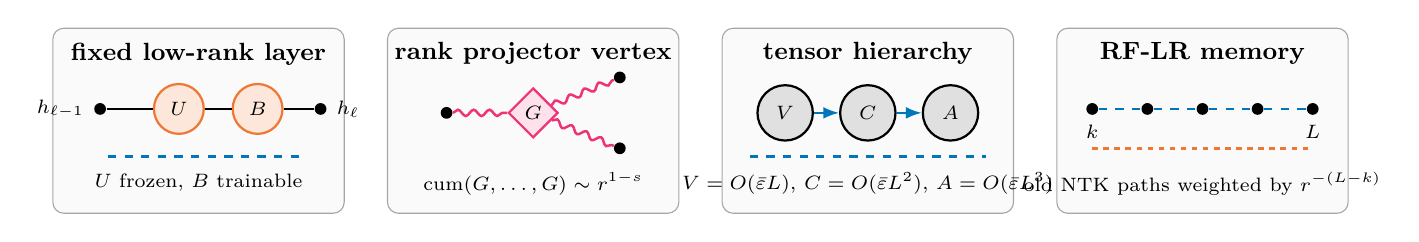
\begin{tikzpicture}[
  x=1cm,
  y=1cm,
  every node/.style={font=\small},
  ext/.style={circle, fill=black, inner sep=1.5pt},
  rankv/.style={circle, draw=color2, fill=color2!18, line width=0.8pt, minimum size=18pt, inner sep=1pt},
  haarv/.style={diamond, draw=color4, fill=color4!14, line width=0.8pt, minimum size=18pt, inner sep=1pt},
  propv/.style={circle, draw=black, fill=white, line width=0.8pt, minimum size=18pt, inner sep=1pt},
  tensorv/.style={circle, draw=black, fill=black!12, line width=0.8pt, minimum size=20pt, inner sep=1pt},
  flow/.style={-{Latex[length=2mm]}, line width=0.8pt},
  nngp/.style={line width=0.9pt},
  ntk/.style={color=color1, dash pattern=on 3pt off 3pt, line width=1pt},
  rankline/.style={color=color2, dash pattern=on 2pt off 2pt, line width=1pt},
  haarline/.style={color=color4, decorate, decoration={snake, amplitude=0.4mm, segment length=2mm}, line width=0.9pt}
]
\node[draw=black!35, rounded corners, fill=black!2, minimum width=3.7cm, minimum height=2.35cm] (p1) at (0,0) {};
\node[font=\bfseries\small] at (0,0.85) {fixed low-rank layer};
\node[ext,label=left:{\scriptsize \(h_{\ell-1}\)}] (h0) at (-1.25,0.15) {};
\node[rankv] (u) at (-0.25,0.15) {\scriptsize \(U\)};
\node[rankv] (b) at (0.75,0.15) {\scriptsize \(B\)};
\node[ext,label=right:{\scriptsize \(h_\ell\)}] (h1) at (1.55,0.15) {};
\draw[nngp] (h0) -- (u) -- (b) -- (h1);
\draw[ntk] (-1.15,-0.45) -- (1.35,-0.45);
\node[font=\scriptsize] at (0,-0.78) {\(U\) frozen, \(B\) trainable};

\node[draw=black!35, rounded corners, fill=black!2, minimum width=3.7cm, minimum height=2.35cm] (p2) at (4.25,0) {};
\node[font=\bfseries\small] at (4.25,0.85) {rank projector vertex};
\node[ext] (g1) at (3.15,0.1) {};
\node[haarv] (g) at (4.25,0.1) {\scriptsize \(G\)};
\node[ext] (g2) at (5.35,0.55) {};
\node[ext] (g3) at (5.35,-0.35) {};
\draw[haarline] (g1) -- (g);
\draw[haarline] (g) -- (g2);
\draw[haarline] (g) -- (g3);
\node[font=\scriptsize] at (4.25,-0.8) {\(\cumul(G,\ldots,G)\sim r^{1-s}\)};

\node[draw=black!35, rounded corners, fill=black!2, minimum width=3.7cm, minimum height=2.35cm] (p3) at (8.5,0) {};
\node[font=\bfseries\small] at (8.5,0.85) {tensor hierarchy};
\node[tensorv] (V) at (7.45,0.1) {\scriptsize \(V\)};
\node[tensorv] (C) at (8.5,0.1) {\scriptsize \(C\)};
\node[tensorv] (A) at (9.55,0.1) {\scriptsize \(A\)};
\draw[flow, color=color1] (V) -- (C);
\draw[flow, color=color1] (C) -- (A);
\draw[ntk] (7.0,-0.45) -- (10.0,-0.45);
\node[font=\scriptsize] at (8.5,-0.8) {\(V=O(\barE L),\,C=O(\barE L^2),\,A=O(\barE L^3)\)};

\node[draw=black!35, rounded corners, fill=black!2, minimum width=3.7cm, minimum height=2.35cm] (p4) at (12.75,0) {};
\node[font=\bfseries\small] at (12.75,0.85) {RF-LR memory};
\node[ext,label=below:{\scriptsize \(k\)}] (m1) at (11.35,0.15) {};
\node[ext] (m2) at (12.05,0.15) {};
\node[ext] (m3) at (12.75,0.15) {};
\node[ext] (m4) at (13.45,0.15) {};
\node[ext,label=below:{\scriptsize \(L\)}] (m5) at (14.15,0.15) {};
\draw[ntk] (m1) -- (m2) -- (m3) -- (m4) -- (m5);
\draw[rankline] (11.35,-0.35) -- (14.15,-0.35);
\node[font=\scriptsize] at (12.75,-0.8) {old NTK paths weighted by \(r^{-(L-k)}\)};
\end{tikzpicture}
}
\caption{Main diagrammatic objects, drawn in the color and line vocabulary used throughout the finite-width NTK diagram literature. Solid black lines denote NNGP/preactivation transport, dashed colored lines denote NTK legs, orange and pink vertices denote rank and Haar-projector cumulants, and gray blobs denote transported tensor cumulants.}
\label{fig:main-diagrammatic-overview}
\end{figure}

\paragraph{Contributions.}
\begin{itemize}[leftmargin=1.4em]
\item We prove exact full-rank matching: at \(r=n\), the factorized network and dense MLP have identical empirical NTKs pathwise.
\item We identify the low-rank Feynman vertices as connected cumulants of \(G=(n/r)UU^\top\), with second cumulant scale \(\gamma_{n,r}\).
\item Under explicit ReLU transport assumptions, we derive tensor scalings \(V=O(\barE L)\), \(C=O(\barE L^2)\), and \(A=O(\barE L^3)\), with endpoint constants \(5\), \(21/20\), and \(173/720\) for isolated off-diagonal modes.
\item Under an explicit well-spread data assumption, we prove operator concentration for finite empirical NTKs at scale \(L^{3/2}\sqrt{m\barE}+mL^3\barE\), up to logarithmic factors, and show that dNTK/ddNTK descendants introduce no new random vertices.
\item We derive a conservative rank-depth stability rule for bottleneck low-rank dynamics: to preserve the centered NTK spectral margin in the unprojected RF-LR model, rank scales cubically with depth, \(r\gtrsim mL^3\), up to logarithmic factors. We also state the separate centered/angularized \(mL^2\) rule with its additional projection hypothesis.
\item We validate the theory with proxy experiments and true finite-network autodiff NTKs, including full-rank matching, rank-defect scaling, operator ratios, and direct cumulant growth.
\end{itemize}

\paragraph{Status of the claims.}
The paper separates what is proved algebraically from what is conditional on standard concentration hypotheses. Full-rank matching, the fixed-left gradient decomposition, the Haar covariance, and the scalar endpoint moments are unconditional calculations. The depth hierarchy and operator bounds are stated under the ReLU edge-of-chaos transport and well-spread data assumptions made explicit below. Direct finite-network cumulants are treated as diagnostics of the polynomial hierarchy, not as direct measurements of isolated Feynman coefficients.

\section{Related Work}
The NTK was introduced as the infinite-width kernel governing gradient-flow training \citep{Jacot2018}. This line of work changed the community's view of overparameterized networks: in the infinite-width lazy regime, training can be studied through a deterministic kernel, and convergence depends on the spectrum of the NTK Gram matrix. Follow-up work showed that wide networks of any depth evolve approximately as linear models around initialization \citep{Lee2019}, and that overparameterized networks can be trained globally under width conditions that keep the empirical NTK stable \citep{Du2019,AllenZhu2019,Arora2019}. These results explain why positive NTK spectra are powerful, but they mostly treat dense networks and do not describe the finite rank-width corrections introduced by factorized layers.

A second thread studies the limits and finite-width corrections of the NTK. Tensor programs give a general language for infinite-width limits and parametrization choices across architectures \citep{Yang2019,Yang2021}. The neural tangent hierarchy and related expansions describe how finite-width dynamics depart from the frozen-kernel limit \citep{Huang2020}. Feynman-diagram methods give a complementary perturbative calculus for wide networks, organizing corrections by connected cumulants and tensor contractions \citep{DyerGurAri2019,FeynmanNTK2026}. Our work follows this finite-width viewpoint, but replaces dense-channel contractions by cumulants of the Haar projector induced by low rank.

The closest optimization and spectral guarantees are complementary rather than substitutive. Prior work proves global convergence for deep networks with one wide layer followed by a pyramidal topology, showing that not every layer must be wide \citep{NguyenMondelli2020}. Tight lower bounds are also known for the smallest eigenvalue of deep ReLU NTKs, including finite-width architectures with one layer of order \(\widetilde\Omega(m)\) and other widths essentially arbitrary \citep{NguyenMondelliMontufar2022}. These results already cover strong ``one wide layer,'' bottleneck-width, global-convergence, and \(\lambda_{\min}\)-type guarantees for full-rank networks. Our claim is different: we do not try to improve their global convergence conditions. We provide a finite-rank perturbation theory for factorized layers \(W=\sqrt{n/r}\,UB\), isolate the exact rank-defect parameter \(\gamma_{n,r}\), prove exact full-rank matching at \(r=n\), and convert the finite-rank NTK deviation into a Weyl spectral-preservation criterion. Recent quantitative GP approximation during training \citep{MosigGarciaAgazziTrevisan2025} is also orthogonal: it controls Wasserstein distance to a Gaussian-process limit for trained shallow networks, whereas our object is operator concentration of \(\wh\Theta-K_*\) for deep low-rank NTKs and the resulting stability of the centered spectral margin.

A third thread concerns practical NTK computation and low-rank structure. Empirical NTKs can be computed efficiently enough to probe finite networks directly \citep{Novak2022}. Low-rank adaptation and low-rank training have also been analyzed in NTK-like regimes, including results showing that sufficiently large low-rank adapters avoid bad local minima in certain settings \citep{Zeng2024LoRA}. These works motivate low rank as an optimization and adaptation tool. Our contribution is different: we ask when low rank preserves the NTK convexity certificate at finite width and finite depth, and we show that the answer depends on whether the rank constraint is an isometric perturbation of the dense MLP or a genuine RF-LR bottleneck.

\section{Models and Full-Rank Matching}
Let \(x_1,\ldots,x_m\) be a fixed dataset. The empirical scalar-output NTK is
\begin{equation}
\wh\Theta_{ab}=\nabla_\theta f(x_a)\cdot \nabla_\theta f(x_b).
\end{equation}
For the factorized model \eqref{eq:intro-model}, trainable parameters are the right factors \(B^{(\ell)}\) and the readout.
We deliberately keep the left Stiefel factors \(U^{(\ell)}\) frozen. This is not only a computational choice. It is what makes the low-rank model a controlled NTK perturbation: the trainable tangent space is a fixed linear subspace, and all rank-dependent randomness enters through the static projector \(G=(n/r)UU^\top\). If \(U\) is trained as well, the tangent space itself moves, producing additional dNTK terms that couple variations of \(U\) and \(B\).

\begin{theorem}[Pathwise full-rank matching]
\label{thm:pathwise}
If \(r_\ell=n_\ell\) for every hidden layer, then for every realization, every dataset, and every depth, the empirical NTK in \(B\)-coordinates equals the empirical NTK of the dense MLP in dense-weight coordinates \(\wt W^{(\ell)}=U^{(\ell)}B^{(\ell)}\). The same equality holds for the NNGP, dNTK, ddNTK, and all tensor cumulants built from them.
\end{theorem}

\begin{proof}
When \(r=n\), \(U\) is orthogonal. The linear map \(\Delta B\mapsto U\Delta B\) preserves Frobenius inner products. The Jacobian with respect to \(B\) is the dense-weight Jacobian composed with this isometry; hence \(J_BJ_B^\top=J_WJ_W^\top\). Higher derivatives and cumulants are invariant under the same coordinate change.
\end{proof}

\begin{proposition}[Why the left factor is frozen]
\label{prop:frozen-left}
Consider one layer \(W=\alpha UB\), with \(U^\top U=I_r\), \(\alpha>0\), and loss gradient \(H=\partial \mathcal L/\partial W\). If only \(B\) is trained, then
\begin{equation}
\nabla_B\mathcal L=\alpha U^\top H,
\qquad
\dot W_B=-\eta\alpha^2UU^\top H.
\label{eq:frozen-left-flow}
\end{equation}
The layer motion is the fixed projected gradient through \(UU^\top\). If \(U\) is also trained on the Stiefel manifold, then the projected Riemannian gradient contributes
\begin{equation}
\dot W_U
=-\eta\alpha^2 (I-UU^\top)H B^\top B
\quad
\text{up to rotations inside } \operatorname{span}(U)\text{ that can be absorbed into }B.
\label{eq:moving-left-flow}
\end{equation}
Consequently the empirical NTK and its time derivative contain additional \(U\)-\(B\) interaction blocks, proportional to contractions with \(B^\top B\). These blocks are absent in the frozen-left model and are not controlled solely by Haar-projector cumulants of \(G=(n/r)UU^\top\).
\end{proposition}

\begin{proof}[Proof idea]
With \(U\) fixed, the only admissible layer variation is \(dW=\alpha U\,dB\), so gradient flow in \(B\) moves the dense weight through the fixed projector \(UU^\top\). If \(U\) is trained, the Stiefel constraint allows normal motions of the subspace in directions \((I-UU^\top)\), and these motions are multiplied by \(B^\top B\) after mapping back to \(W=\alpha UB\). Thus the tangent kernel is no longer a fixed-projector \(B\)-kernel: it contains moving-subspace and \(U/B\) cross blocks. The full differential calculation is given in Appendix \ref{app:frozen-left-full-proof}.
\end{proof}

Proposition \ref{prop:frozen-left} explains the modeling choice. Training both factors may be useful in practice, but it is a different dynamical system: the low-rank subspace rotates during training, and the NTK drift receives extra moving-projector terms. Freezing \(U\) isolates the rank-width effect we can prove and keeps the diagrammatics closed under the Haar projector vertices of Lemma \ref{lem:haar-cov}.

The RF-LR bottleneck has a different recursion,
\begin{equation}
\Theta^{(\ell)}=1+\frac1r\Theta^{(\ell-1)}\dot\Sigma^{(\ell)}+\frac1r\Sigma^{(\ell)}.
\label{eq:rflr-recursion}
\end{equation}
At the ReLU fixed point \(\dot\Sigma^{(\ell)}\to1/2\), so an old NTK contribution is multiplied by approximately \((2r)^{-(L-k)}\). This is a different model, not a perturbation of the dense MLP.

\section{Haar Projector Vertices}
Let \(U\in\R^{n\times r}\) be Haar-Stiefel and \(G=(n/r)UU^\top\). Orthogonal invariance gives the full covariance tensor.

\begin{lemma}[Haar projector covariance]
\label{lem:haar-cov}
For all indices,
\begin{equation}
\Cov(G_{ij},G_{kl})=\gamma_{n,r}\left(\delta_{ik}\delta_{jl}+\delta_{il}\delta_{jk}-\frac2n\delta_{ij}\delta_{kl}\right),
\qquad
\gamma_{n,r}=\frac{n(n-r)}{r(n-1)(n+2)}.
\label{eq:haar-cov}
\end{equation}
In particular \(\gamma_{n,n}=0\).
\end{lemma}

\begin{proof}
The covariance of a Haar projector has the invariant form \(a(\delta_{ik}\delta_{jl}+\delta_{il}\delta_{jk})+b\delta_{ij}\delta_{kl}\). The identity \(\tr G=n\) gives \(2a+nb=0\). The standard second moment of a Haar projector gives \(a=\gamma_{n,r}\), hence \eqref{eq:haar-cov}.
\end{proof}

Higher cumulants are given by orthogonal Weingarten contractions. Connected \(s\)-point cumulants scale as \(O_s(r^{1-s})\) and vanish in the full-rank endpoint. Thus the low-rank Feynman rule is simple: dense Gaussian-ReLU vertices remain, and each low-rank correction inserts connected cumulants of \(G\).

\begin{lemma}[Rank cumulant power counting]
\label{lem:rank-cumulant-counting}
Fix a layer \(\ell\) and condition on all previous layers. For rank channel \(a\), let
\[
Z_a^{(\ell)}
:=
\left\{
\bigl(g_a^{(\ell)}(x_u),\sigma(g_a^{(\ell)}(x_u)),\sigma'(g_a^{(\ell)}(x_u))\bigr)_{u=1}^{m},
\text{ and the corresponding derivative atoms}
\right\}.
\]
Here \(g_a^{(\ell)}(x_u)\) is the scalar preactivation of rank channel \(a\) on sample \(x_u\), after the deterministic conditioning on layer \(\ell-1\). Thus \(Z_a^{(\ell)}\) is the full local random object from which one-channel quantities such as \(\sigma\sigma\), \(\sigma\sigma'\), \(\sigma'\sigma'\), and derivative insertions are evaluated. The variables \(Z_1^{(\ell)},\ldots,Z_r^{(\ell)}\) are conditionally iid. To simplify notation, write them as \(Z_a\), and assume the local functions below have uniformly bounded moments of all orders. Define empirical observables
\[
X_i^{(r)}=r^{-a_i}\sum_{a=1}^{r} f_i(Z_a),
\qquad i=1,\ldots,s.
\]
Then the connected cumulant satisfies
\begin{equation}
\cumul\left(X_1^{(r)},\ldots,X_s^{(r)}\right)
=r^{1-\sum_i a_i}\,
\cumul\left(f_1(Z),\ldots,f_s(Z)\right).
\label{eq:rank-cumulant-counting}
\end{equation}
In particular, normalized empirical averages have \(s\)-point cumulants of order \(r^{1-s}\).
\end{lemma}

\begin{proof}
By multilinearity of cumulants,
\[
\cumul(X_1^{(r)},\ldots,X_s^{(r)})
=r^{-\sum_i a_i}
\sum_{a_1,\ldots,a_s=1}^{r}
\cumul(f_1(Z_{a_1}),\ldots,f_s(Z_{a_s})).
\]
Independence kills every term whose indices are not all in the same connected block. Only \(a_1=\cdots=a_s\) contributes, giving \(r\) identical terms and hence \eqref{eq:rank-cumulant-counting}.
\end{proof}

This elementary lemma is the right-factor-only analogue of the usual width power counting. It explains why finite-rank bias terms are typically \(O(r^{-1})\) after averaging over seeds, while single-seed fluctuations are \(O_{\Pp}(r^{-1/2})\). It also explains why the exact full-rank endpoint must be treated with the projector defect \(G-I\), rather than by the informal replacement \(n\mapsto r\).

\section{Tensor Scaling at ReLU Edge of Chaos}
For normalized ReLU, the edge-of-chaos correlation asymptotics used in the RF-LR analysis \citep{RFLR2026} give
\(\theta_\ell=3\pi/\ell+O(\log \ell/\ell^2)\), and
\begin{equation}
\dot{\mathcal C}(\rho_\ell)=1-\frac3\ell+O\left(\frac{\log\ell}{\ell^2}\right).
\label{eq:relu-transport}
\end{equation}
Transporting an external NTK leg from layer \(k\) to \(L\) gives the factor \((k/L)^\lambda\) for an exponent \(\lambda\in\{0,3\}\), depending on whether the Gram entry is diagonal or off-diagonal.

\begin{lemma}[Depth-transport accumulation]
\label{lem:transport-source}
Let \(T_\ell\in\R^d\) satisfy
\begin{equation}
T_{\ell+1}
=\left(I-\frac{M}{\ell}+E_\ell\right)T_\ell+\ell^\beta(s+e_\ell),
\label{eq:transport-source-recursion}
\end{equation}
where \(\norm{E_\ell}\le C\log^p(\ell)/\ell^2\), \(\norm{e_\ell}\le C\log^q(\ell)/\ell\), and \(M+(\beta+1)I\) is invertible. Then
\begin{equation}
T_L
=L^{\beta+1}\left(M+(\beta+1)I\right)^{-1}s
+O\left(L^\beta\log^{p+q+2}L\right).
\label{eq:transport-source-solution}
\end{equation}
\end{lemma}

\begin{proof}
Iterating \eqref{eq:transport-source-recursion} gives a variation-of-constants formula. The product of propagators from \(k\) to \(L\) is \((k/L)^M\) up to a multiplicative error whose accumulated contribution is \(O(L^\beta\log^{p+q+2}L)\), since \(\sum_k\log^p(k)/k^2<\infty\). Thus
\[
T_L=L^{-M}\sum_{k\le L} k^{M+\beta I}s+O(L^\beta\log^{p+q+2}L).
\]
Euler-Maclaurin yields
\[
L^{-M}\sum_{k\le L} k^{M+\beta I}
=L^{\beta+1}\int_0^1u^{M+\beta I}\,\dd u+O(L^\beta),
\]
and the matrix integral is \((M+(\beta+1)I)^{-1}\).
\end{proof}

Let \(\barE=\max_{\ell\le L}(1/n_\ell+\gamma_{n_\ell,r_\ell})\). The finite-width tensors obey
\begin{equation}
V_L=O(\barE L),\qquad C_L=O(\barE L^2),\qquad A_L=O(\barE L^3),
\label{eq:main-scales}
\end{equation}
where \(C\) denotes the mixed NNGP-NTK block \((D,F)\), and \(A\) denotes the NTK-NTK block \((A,B)\).

\begin{proposition}[Conditional tensor hierarchy]
\label{prop:tensor-hierarchy}
Assume the low-rank cumulant recursion closes on the same tensor sectors as the dense finite-width Feynman hierarchy and that the ReLU edge-of-chaos transport is uniform away from the diagonal singularity. Then the isolated tensor coordinates satisfy
\begin{equation}
V_L=O(\barE L),\qquad
D_L,F_L=O(\barE L^2),\qquad
A_L,B_L=O(\barE L^3).
\label{eq:tensor-hierarchy}
\end{equation}
Consequently, the perturbative mean-NTK correction is controlled in the regime \(L^3\barE\ll 1\).
\end{proposition}

\begin{proof}
The fresh NNGP four-point source contributes \(O(\barE)\) per layer and has no transported NTK leg in the dominant radial mode, so summation gives \(V_L=O(\barE L)\). The mixed blocks \(D,F\) have one transported NTK leg and therefore one depth-transport accumulation with \(\beta=1\), yielding \(O(\barE L^2)\) by Lemma \ref{lem:transport-source}. The NTK-NTK blocks \(A,B\) have two transported NTK legs, equivalently source exponent \(\beta=2\), giving \(O(\barE L^3)\). These are isolated tensor coordinates; scalar-output cumulants can mix these sectors.
\end{proof}

\paragraph{Endpoint constants.}
At the ReLU endpoint, set \(X_0=2(g_+)^2\) and \(Y_0=2\one_{\{g>0\}}\). Then
\begin{equation}
\Var(X_0)=5,
\qquad
\Cov(X_0,Y_0)=1,
\qquad
\Var(Y_0)=1.
\end{equation}
The three constants correspond to the following endpoint diagrams:
\begin{figure}[t]
\centering
\resizebox{0.92\linewidth}{!}{%
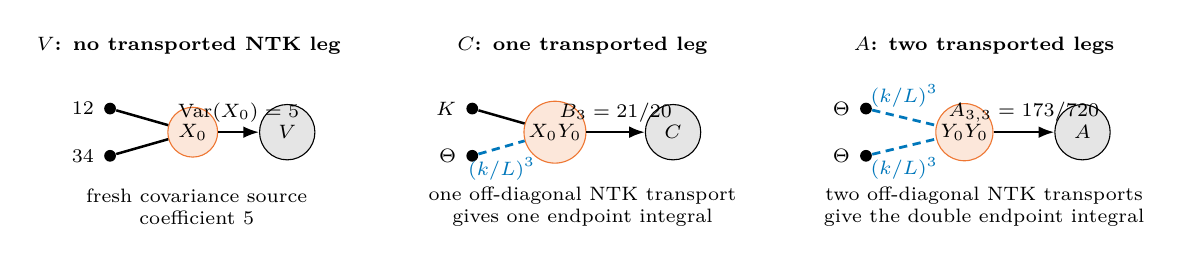
\begin{tikzpicture}[
  x=1cm,
  y=1cm,
  ext/.style={circle, fill=black, inner sep=1.5pt},
  nngp/.style={line width=0.9pt},
  ntk/.style={color=color1, dash pattern=on 3pt off 2pt, line width=1pt},
  src/.style={circle, draw=color2, fill=color2!18, minimum size=18pt, inner sep=1pt},
  tensor/.style={circle, draw=black, fill=black!10, minimum size=20pt, inner sep=1pt},
  flow/.style={-{Latex[length=2mm]}, line width=0.75pt},
  every node/.style={font=\small}
]
\node[font=\bfseries\scriptsize] at (0,1.05) {\(V\): no transported NTK leg};
\node[ext,label=left:{\scriptsize \(12\)}] (v1) at (-1,0.25) {};
\node[ext,label=left:{\scriptsize \(34\)}] (v2) at (-1,-0.35) {};
\node[src] (vs) at (0.05,-0.05) {\scriptsize \(X_0\)};
\node[tensor] (vt) at (1.25,-0.05) {\scriptsize \(V\)};
\draw[nngp] (v1) -- (vs);
\draw[nngp] (v2) -- (vs);
\draw[flow] (vs) -- node[above,font=\scriptsize] {\(\Var(X_0)=5\)} (vt);
\node[font=\scriptsize, align=center] at (0.1,-1.0) {fresh covariance source\\coefficient \(5\)};

\node[font=\bfseries\scriptsize] at (5.0,1.05) {\(C\): one transported leg};
\node[ext,label=left:{\scriptsize \(K\)}] (c1) at (3.6,0.25) {};
\node[ext,label=left:{\scriptsize \(\Theta\)}] (c2) at (3.6,-0.35) {};
\node[src] (cs) at (4.65,-0.05) {\scriptsize \(X_0Y_0\)};
\node[tensor] (ct) at (6.15,-0.05) {\scriptsize \(C\)};
\draw[nngp] (c1) -- (cs);
\draw[ntk] (c2) -- node[below,font=\scriptsize] {\((k/L)^3\)} (cs);
\draw[flow] (cs) -- node[above,font=\scriptsize] {\(B_3=21/20\)} (ct);
\node[font=\scriptsize, align=center] at (5.0,-1.0) {one off-diagonal NTK transport\\gives one endpoint integral};

\node[font=\bfseries\scriptsize] at (10.1,1.05) {\(A\): two transported legs};
\node[ext,label=left:{\scriptsize \(\Theta\)}] (a1) at (8.6,0.25) {};
\node[ext,label=left:{\scriptsize \(\Theta\)}] (a2) at (8.6,-0.35) {};
\node[src] (as) at (9.85,-0.05) {\scriptsize \(Y_0Y_0\)};
\node[tensor] (at) at (11.35,-0.05) {\scriptsize \(A\)};
\draw[ntk] (a1) -- node[above,font=\scriptsize] {\((k/L)^3\)} (as);
\draw[ntk] (a2) -- node[below,font=\scriptsize] {\((k/L)^3\)} (as);
\draw[flow] (as) -- node[above,font=\scriptsize] {\(A_{3,3}=173/720\)} (at);
\node[font=\scriptsize, align=center] at (10.1,-1.0) {two off-diagonal NTK transports\\give the double endpoint integral};
\end{tikzpicture}
}
\caption{Endpoint diagrams for the constants in \eqref{eq:endpoint-constants}. A \(V\)-source has no transported NTK leg and gives \(\Var(X_0)=5\). A mixed \(C\)-diagram has one off-diagonal NTK leg transported by \((k/L)^3\), giving \(B_3=21/20\). An \(A\)-diagram has two such transported legs, giving \(A_{3,3}=173/720\).}
\label{fig:endpoint-constant-diagrams}
\end{figure}
For a transported off-diagonal leg, \(\lambda=3\). Indeed, the leg is multiplied from layer \(k\) to layer \(L\) by
\[
\prod_{j=k+1}^{L}\dot{\mathcal C}(\rho_j)
=\prod_{j=k+1}^{L}\left(1-\frac3j+O\left(\frac{\log j}{j^2}\right)\right)
=\left(\frac{k}{L}\right)^3(1+o(1)),
\]
because the logarithm of the product is \(-3\sum_{j=k+1}^{L}j^{-1}+O(1/k)\). This is the source of the exponent \(3\). The mixed and NTK-NTK endpoint integrals are
\begin{equation}
B_\lambda=\frac1{\lambda+1}\left(5-\frac4{\lambda+2}\right),
\qquad
A_{\lambda,\mu}=\frac{1}{(\lambda+1)(\mu+1)}\left(5-\frac4{\lambda+2}-\frac4{\mu+2}+\frac4{\lambda+\mu+3}\right).
\end{equation}
Thus for off-diagonal modes,
\begin{equation}
V: 5,
\qquad
C: B_3=\frac{21}{20},
\qquad
A: A_{3,3}=\frac{173}{720}.
\label{eq:endpoint-constants}
\end{equation}

These constants are tensor coefficients after pairing-basis extraction, not arbitrary scalar-output cumulants. Direct finite-network cumulants mix Wick/Wishart terms, radial modes, readout contractions, and several Feynman sectors; they are therefore expected to show finite-depth effective slopes rather than the isolated constants exactly.

\subsection{A three-layer finite-rank calculation}
The simplest place where the low-rank simplification is visible is a three-layer network, i.e. two ReLU feature maps. Let
\[
Q_x=\frac1r\sum_{a=1}^{r}X_a^2,\qquad
Q_y=\frac1r\sum_{a=1}^{r}Y_a^2,\qquad
S=\frac1r\sum_{a=1}^{r}X_aY_a,
\qquad
C_r=\frac{S}{\sqrt{Q_xQ_y}}.
\]
For the right-factor-only low-rank model, the empirical second hidden-layer kernel has the schematic form
\[
K_{2,r}=\sqrt{Q_xQ_y}\,\kappa(C_r),
\qquad
\dot K_{2,r}=\dot\kappa(C_r),
\qquad
\wh\Theta^{(3)}_r=K_{2,r}+S\,\dot K_{2,r},
\]
where \(\kappa\) is the normalized ReLU covariance map.

\begin{proposition}[Delta-method correction for three layers]
\label{prop:three-layer-delta}
For fixed correlation \(\rho\in(-1,1)\), there is an explicit smooth function \(\Delta^{(3)}(\rho)\), depending only on \(\kappa,\dot\kappa\) and the covariance matrix of \((X^2,Y^2,XY)\), such that
\begin{equation}
\E\,\wh\Theta^{(3)}_r(\rho)
=\Theta^{(3)}_\infty(\rho)+\frac1r\Delta^{(3)}(\rho)+O(r^{-2}),
\qquad
\wh\Theta^{(3)}_r-\E\wh\Theta^{(3)}_r=O_{\Pp}(r^{-1/2}).
\label{eq:three-layer-delta}
\end{equation}
For scale-invariant ReLU on the diagonal, \(\Delta^{(3)}(1)=0\).
\end{proposition}

\begin{proof}
Write \(\wh\Theta^{(3)}_r=F(Q_x,Q_y,S)\). By the multivariate central limit theorem and Lemma \ref{lem:rank-cumulant-counting},
\[
(Q_x,Q_y,S)=(1,1,\rho)+r^{-1/2}\xi+O_{\Pp}(r^{-1})
\]
with \(\xi\) asymptotically Gaussian and covariance determined by the moments of \((X^2,Y^2,XY)\). Taylor expansion gives
\[
\E F(Q_x,Q_y,S)
=F(1,1,\rho)+\frac1{2r}\tr\left(\nabla^2F(1,1,\rho)\,\Sigma_\rho\right)+O(r^{-2}),
\]
which is \eqref{eq:three-layer-delta}. The \(O_{\Pp}(r^{-1/2})\) fluctuation is the first-order delta-method term. On the diagonal \(X=Y\), ReLU scale invariance makes the normalized correlation and derivative atoms deterministic along the radial direction, cancelling the first mean correction.
\end{proof}

\section{Operator Concentration and Spectral Preservation}
Let \(\Theta_{\infty,L}\) be the deterministic limiting NTK and \(\wh\Theta_L\) the empirical finite NTK. Entrywise tensor bounds give
\begin{equation}
\Var((\wh\Theta_L)_{ab})\lesssim L^3\barE,
\qquad
|\E(\wh\Theta_L)_{ab}-(\Theta_{\infty,L})_{ab}|\lesssim L^3\barE.
\end{equation}
A layer martingale and matrix Freedman yield the operator form. The well-spread data assumption below means that no small group of examples dominates the random feature directions; equivalently, the matrix variance of the empirical NTK fluctuation grows like \(m\), not \(m^2\).

\begin{theorem}[Finite-network operator concentration]
\label{thm:operator}
Assume \(L^3\barE\le c\). Assume further that the data are well-spread in the layerwise feature bases, so the entrywise tensor variance bounds upgrade to a matrix variance proxy of order \(mL^3\barE\). With probability at least \(1-\delta\),
\begin{equation}
\|\wh\Theta_L-\Theta_{\infty,L}\|_{\op}
\le
C L^{3/2}\sqrt{m\barE}\,\operatorname{polylog}(m,L,1/\delta)
+C mL^3\barE\,\operatorname{polylog}(m,L,1/\delta).
\label{eq:operator-bound}
\end{equation}
A robust version replaces the first term by \(C mL^{3/2}\sqrt{\barE}\) without the well-spread data assumption.
\end{theorem}

\begin{proof}[Proof sketch]
Expose the random weights and projectors layer by layer and decompose \(\wh\Theta_L-\E\wh\Theta_L\) as a matrix martingale. Proposition \ref{prop:tensor-hierarchy} gives conditional entrywise variance \(O(L^3\barE)\) and conditional bias \(O(L^3\barE)\). Under the well-spread data assumption, the predictable quadratic variation is \(O(mL^3\barE)\) in operator norm rather than \(O(m^2L^3\barE)\). Matrix Freedman gives the first term in \eqref{eq:operator-bound}, with logarithmic losses from truncation and union over tensor coordinates. The deterministic bias contributes the second term. Without this assumption, the same argument uses the Frobenius-to-operator bound on the variance proxy and loses a factor \(\sqrt m\).
\end{proof}

If \(\mu_\infty(L)=\lambda_{\min}(P_m\Theta_{\infty,L}P_m)\) is the limiting centered spectral margin, Weyl's inequality gives preservation whenever the right-hand side of \eqref{eq:operator-bound} is at most \(\mu_\infty(L)/2\). In the RF-LR bottleneck, the baseline is not the dense MLP margin; the centered proxy margin can scale as \(1/(rL)\). Combining this with the bottleneck deviation gives the conservative design rule \(r\gtrsim mL^3\), up to logarithmic factors, when the RF-LR perturbation scale is \(1/r\).

\subsection{RF-LR memory and rank-depth rules}
The RF-LR recursion \eqref{eq:rflr-recursion} is not a full-rank-compatible perturbation. Its old-kernel memory obeys an exact product rule:
\begin{equation}
\Theta^{(L)}_{\mathrm{old}\leftarrow k}
=\Theta^{(k)}\prod_{j=k+1}^{L}\frac{\dot\Sigma^{(j)}}{r}.
\label{eq:rflr-memory-product}
\end{equation}
At the normalized ReLU edge of chaos, \(\dot\Sigma^{(j)}=1/2+O(j^{-1})\), hence
\begin{equation}
\left|\Theta^{(L)}_{\mathrm{old}\leftarrow k}\right|
\le C\left(\frac1{2r}\right)^{L-k}\left(\frac{L}{k}\right)^C.
\label{eq:rflr-memory-bound}
\end{equation}
Low rank therefore shortens old NTK memory geometrically. The cost is that the centered deterministic margin can shrink with \(r\) and \(L\).

\begin{proposition}[Unprojected and centered RF-LR stability rules]
\label{prop:rflr-rules}
Consider an RF-LR bottleneck whose centered limiting margin satisfies
\(\mu_{\mathrm{RF}}(L,r)\gtrsim (rL)^{-1}\). If the empirical operator deviation is controlled by the conservative scale \(L^{3/2}\sqrt{m/r}+mL^3/r\), then spectral preservation follows from
\begin{equation}
r\gtrsim mL^3\,\operatorname{polylog}(m,L,1/\delta).
\label{eq:rflr-unprojected-rule}
\end{equation}
If the radial mode is projected out and an angularized centered decomposition improves the variance scale by one power of \(L\), then the sufficient rule improves to
\begin{equation}
r\gtrsim mL^2\,\operatorname{polylog}(m,L,1/\delta).
\label{eq:rflr-centered-rule}
\end{equation}
\end{proposition}

\begin{proof}
Weyl's inequality requires the operator deviation to be at most a fixed fraction of \(\mu_{\mathrm{RF}}(L,r)\). In the unprojected RF-LR model, the radial contribution remains present in the \(A\)-sector, whose tensor scale is cubic in depth. The sufficient inequality is therefore dominated by the \(mL^3/r\) contribution after absorbing logarithms and constants, giving \eqref{eq:rflr-unprojected-rule}. In the centered/angularized model, the radial sector is removed before concentration and the dominant tensor variance is quadratic in depth. Repeating the same Weyl argument gives \eqref{eq:rflr-centered-rule}. The second statement is conditional on this projection and should not be read as the default RF-LR rule.
\end{proof}

\section{NTK Descendants and Training-Time Drift}
Let \(J_c=\nabla_\theta f(x_c)\) and define the dNTK and ddNTK descendants
\begin{equation}
\Xi_{ab;c}=D\Theta_{ab}[J_c],
\qquad
\Psi_{ab;cd}=D^2\Theta_{ab}[J_c,J_d].
\end{equation}
These descendants add derivative legs to the same layer maps. They do not introduce new independent random variables.

\begin{proposition}[No new low-rank vertices]
\label{prop:no-new-vertices}
The joint cumulants of \((K,\Theta,\Xi,\Psi)\) are generated by the same Gaussian-ReLU atoms and Haar-projector cumulants of \(G=(n/r)UU^\top\). Differentiation changes deterministic contractions but not the probabilistic vertex set.
\end{proposition}

\begin{proof}
Each derivative of the network output with respect to a trainable right factor \(B^{(\ell)}\) inserts an additional deterministic backpropagated leg and a factor of the same frozen projector \(UU^\top\). Higher derivatives differentiate ReLU gates and covariance maps, changing the local deterministic tensors \(\kappa,\dot\kappa,\ddot\kappa\), but all randomness still comes from the original Gaussian preactivations, readout weights, and frozen projectors. Since \(U\) is fixed, there is no moving-projector derivative. Thus the connected diagrams for \(K,\Theta,\Xi,\Psi\) have the same random vertices as the NTK diagrams and only differ in their deterministic leg labels.
\end{proof}

Under square-loss gradient flow, \(\dot\Theta_{ab,t}=-\sum_c\Xi_{ab;c,t}e_{c,t}\). The descendant concentration bound therefore yields, in a lazy window,
\begin{equation}
\|\Theta_t-\Theta_0\|_{\op}
\le
C t\|e_0\|_2\left(L^3\sqrt{m\barE}+mL^3\barE\right)\operatorname{polylog}(m,L,1/\delta).
\end{equation}

\section{Experiments}
We run three classes of experiments and present the figures in the same order as the theory. Proxy experiments first validate the rank-projector law and operator normalization. We then check the endpoint tensor constants and RF-LR memory suppression. Finally, true finite-network experiments compute empirical NTKs by PyTorch autograd and estimate direct finite-network covariances of the NNGP Gram and empirical NTK.

\begin{figure}[t]
\centering
\begin{minipage}{0.32\linewidth}
\centering
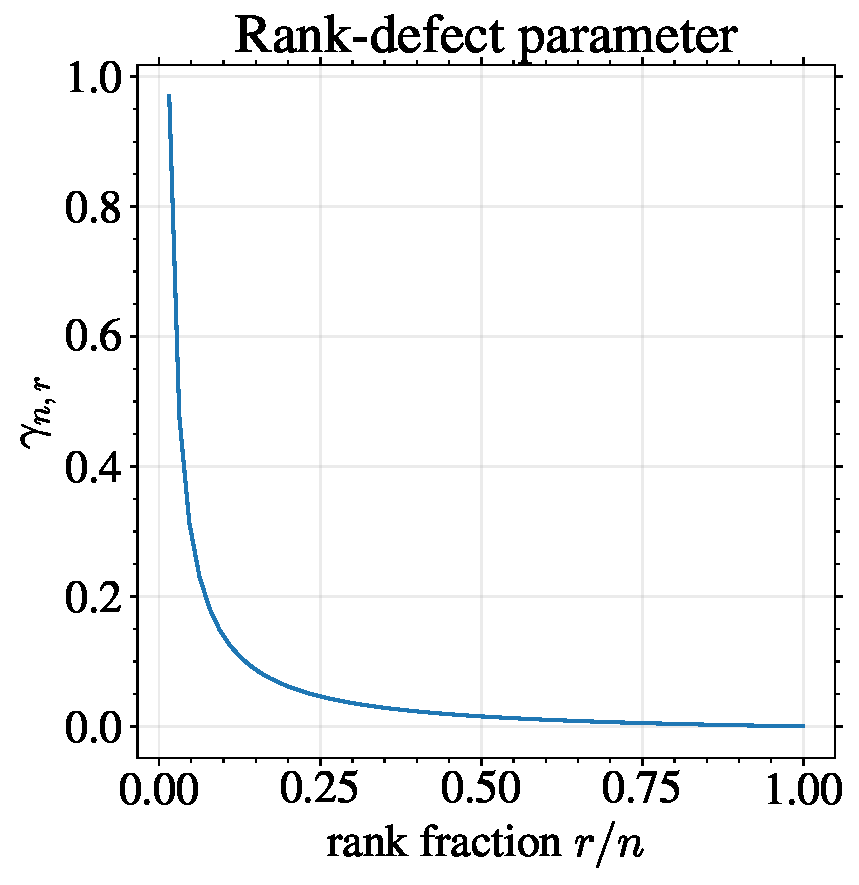
\includegraphics[width=\linewidth]{../../data/feynman/lowrank_ntk_proxy_outputs_clean/rank_defect_gamma.pdf}
\end{minipage}
\hfill
\begin{minipage}{0.32\linewidth}
\centering
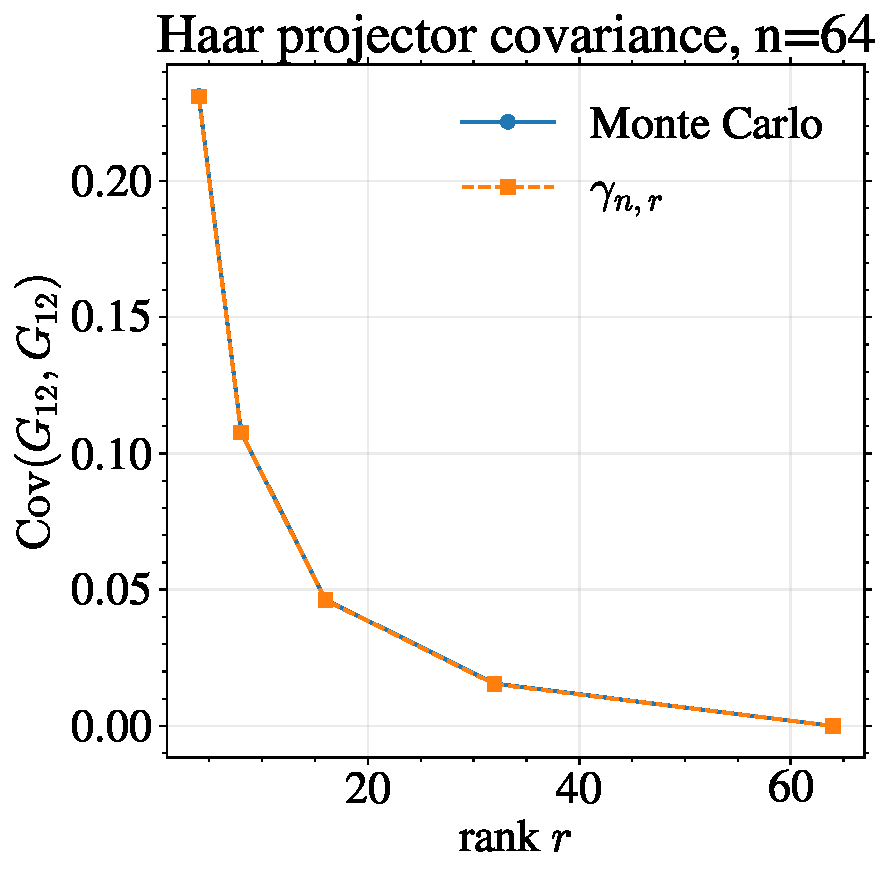
\includegraphics[width=\linewidth]{../../data/feynman/lowrank_ntk_proxy_outputs_clean/haar_covariance.pdf}
\end{minipage}
\hfill
\begin{minipage}{0.32\linewidth}
\centering
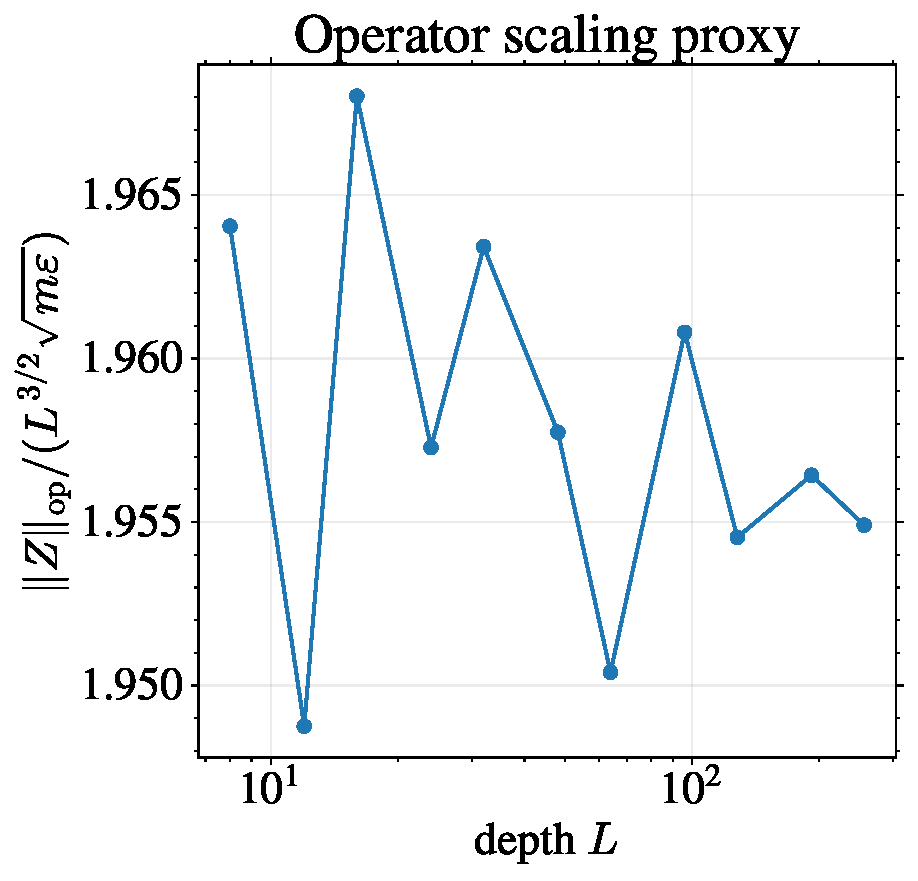
\includegraphics[width=\linewidth]{../../data/feynman/lowrank_ntk_proxy_outputs_clean/operator_proxy_ratio.pdf}
\end{minipage}
\caption{Rank-projector and operator checks. Left: the rank-defect scale \(\gamma_{n,r}\) vanishes at full rank. Middle: empirical Haar-projector covariance matches the closed form. Right: the normalized operator proxy \(\|Z\|_{\op}/(L^{3/2}\sqrt{m\eps})\) is approximately stable across depth.}
\label{fig:proxy-haar-operator}
\end{figure}

\begin{figure}[t]
\centering
\begin{minipage}{0.24\linewidth}
\centering
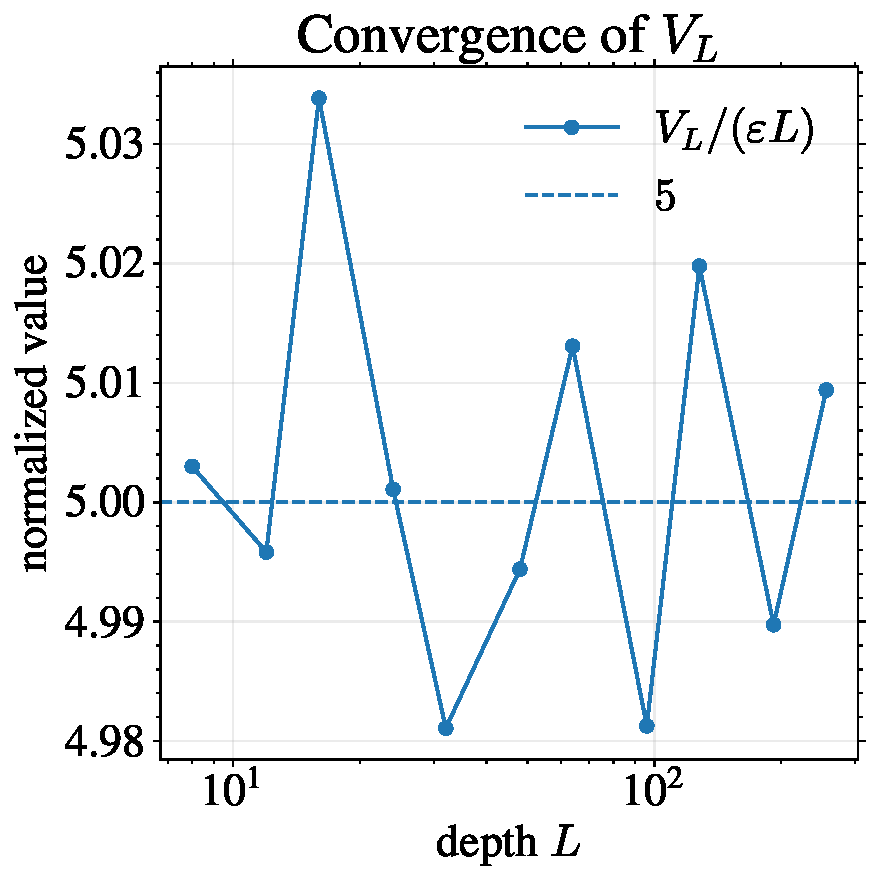
\includegraphics[width=\linewidth]{../../data/feynman/lowrank_ntk_proxy_outputs_clean/convergence_V.pdf}
\end{minipage}
\hfill
\begin{minipage}{0.24\linewidth}
\centering
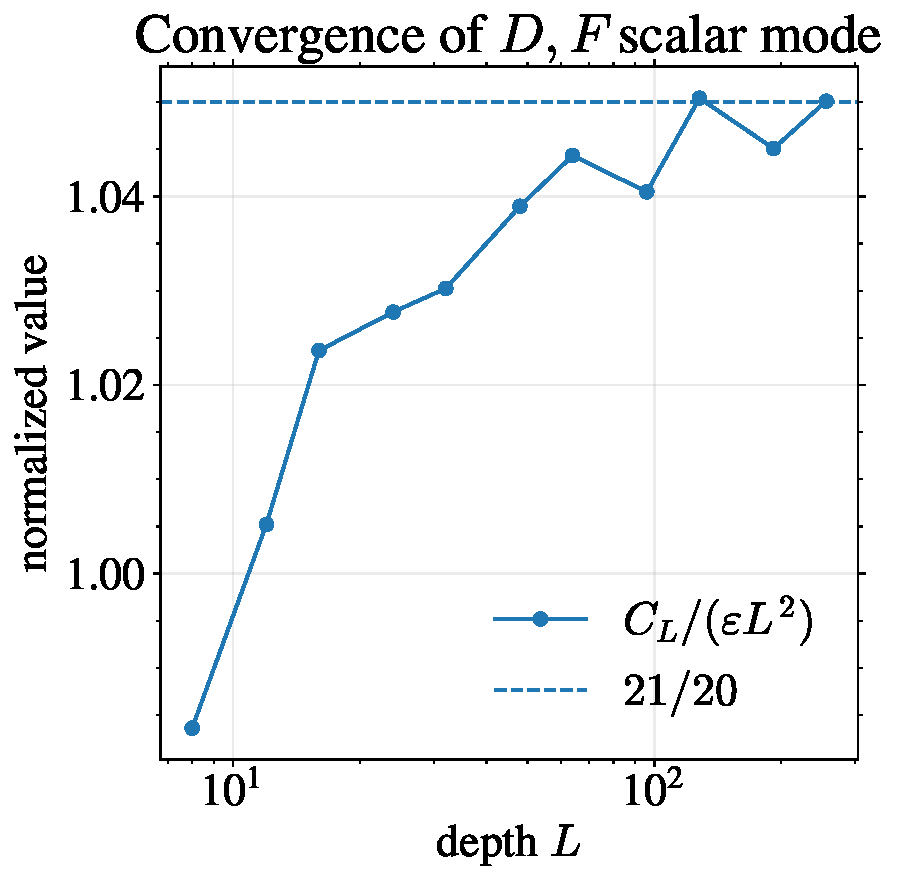
\includegraphics[width=\linewidth]{../../data/feynman/lowrank_ntk_proxy_outputs_clean/convergence_C.pdf}
\end{minipage}
\hfill
\begin{minipage}{0.24\linewidth}
\centering
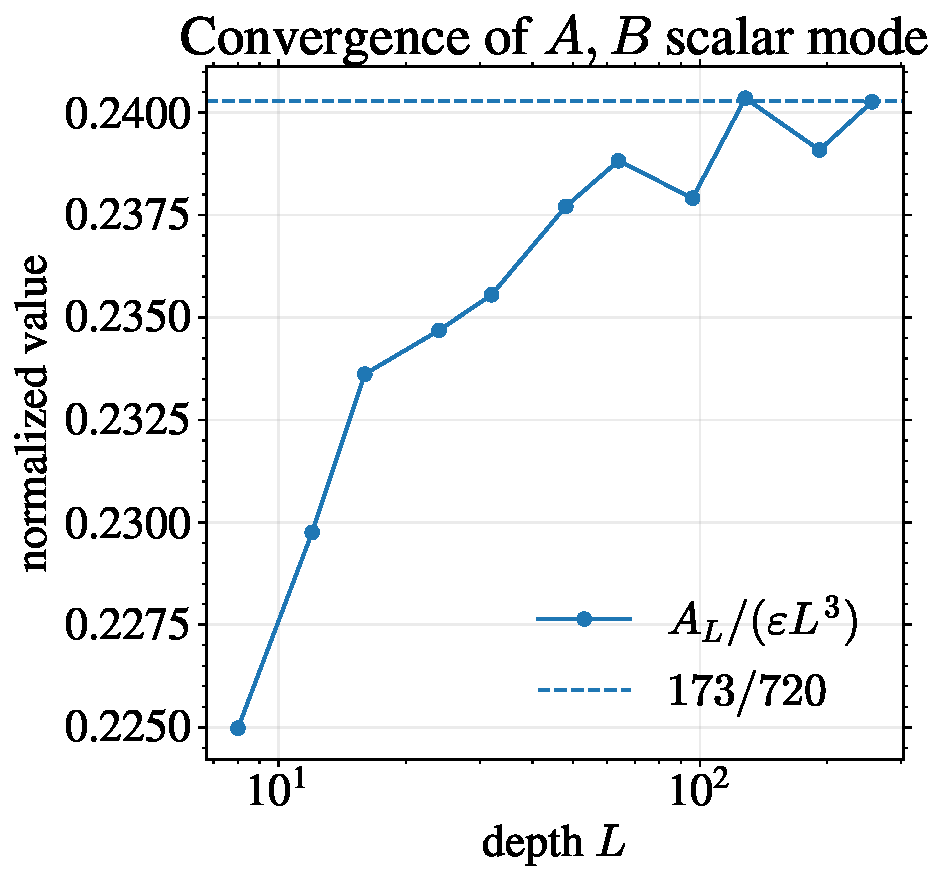
\includegraphics[width=\linewidth]{../../data/feynman/lowrank_ntk_proxy_outputs_clean/convergence_A.pdf}
\end{minipage}
\hfill
\begin{minipage}{0.24\linewidth}
\centering
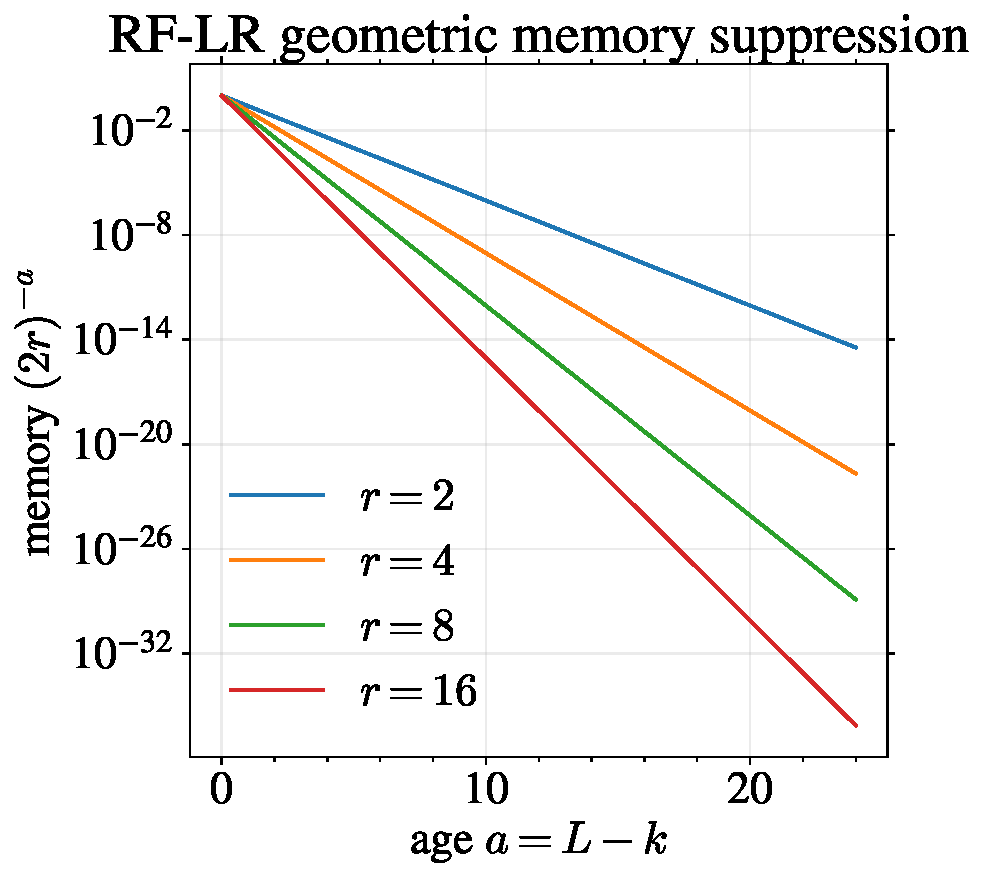
\includegraphics[width=\linewidth]{../../data/feynman/lowrank_ntk_proxy_outputs_clean/rflr_memory_suppression.pdf}
\end{minipage}
\caption{Tensor constants and RF-LR memory. The first three panels show convergence to the isolated constants \(5\), \(21/20\), and \(173/720\). The last panel shows geometric suppression of old NTK memory in the RF-LR bottleneck.}
\label{fig:proxy-constants}
\end{figure}

\begin{figure}[t]
\centering
\begin{minipage}{0.48\linewidth}
\centering
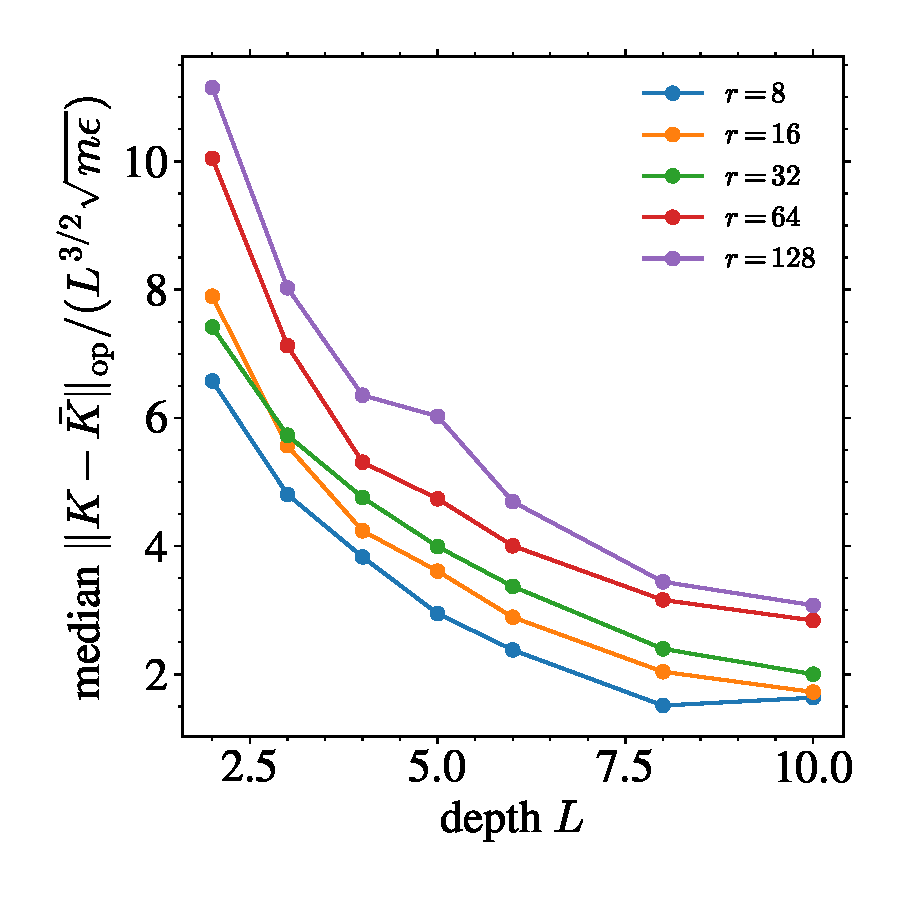
\includegraphics[width=\linewidth]{../../data/feynman/true_finite_ntk_outputs_clean/true_finite_ntk_operator_ratio.pdf}
\end{minipage}
\hfill
\begin{minipage}{0.48\linewidth}
\centering
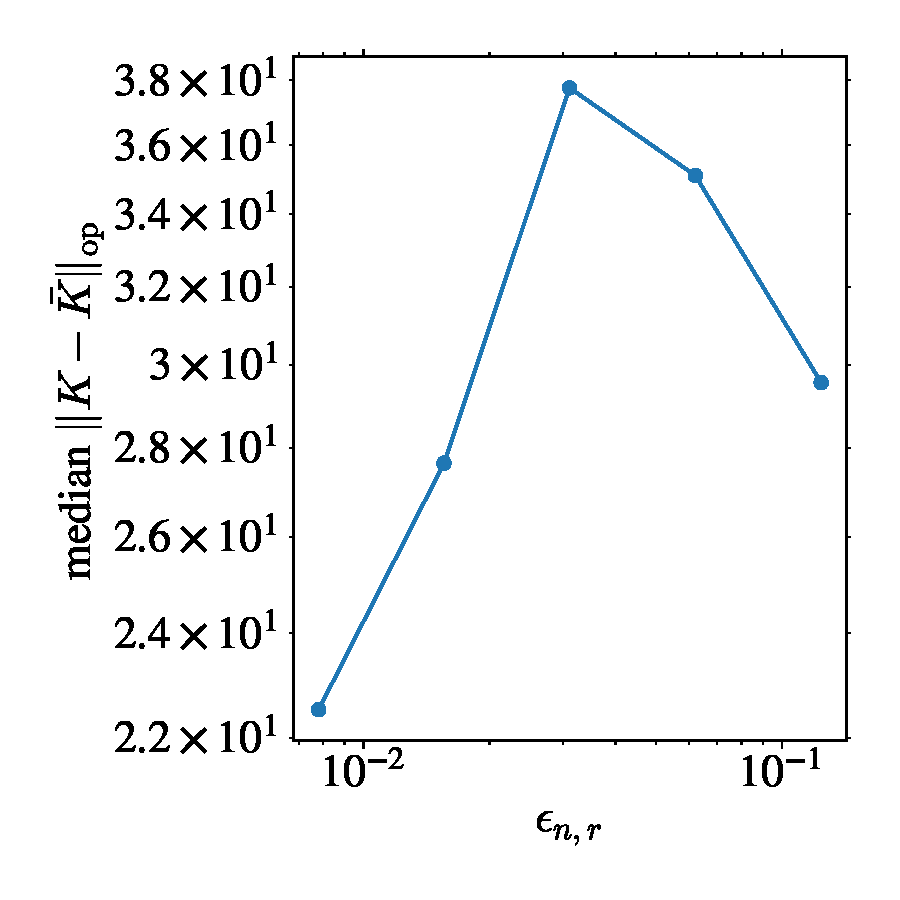
\includegraphics[width=\linewidth]{../../data/feynman/true_finite_ntk_outputs_clean/true_finite_ntk_rank_defect_scaling.pdf}
\end{minipage}
\caption{True finite-network NTK checks computed by autodiff. Left: empirical operator deviations follow the predicted normalization. Right: the finite-network deviation tracks the rank-defect scale and vanishes at the full-rank endpoint.}
\label{fig:true-ntk-operator-rank}
\end{figure}

\begin{figure}[t]
\centering
\begin{minipage}{0.32\linewidth}
\centering
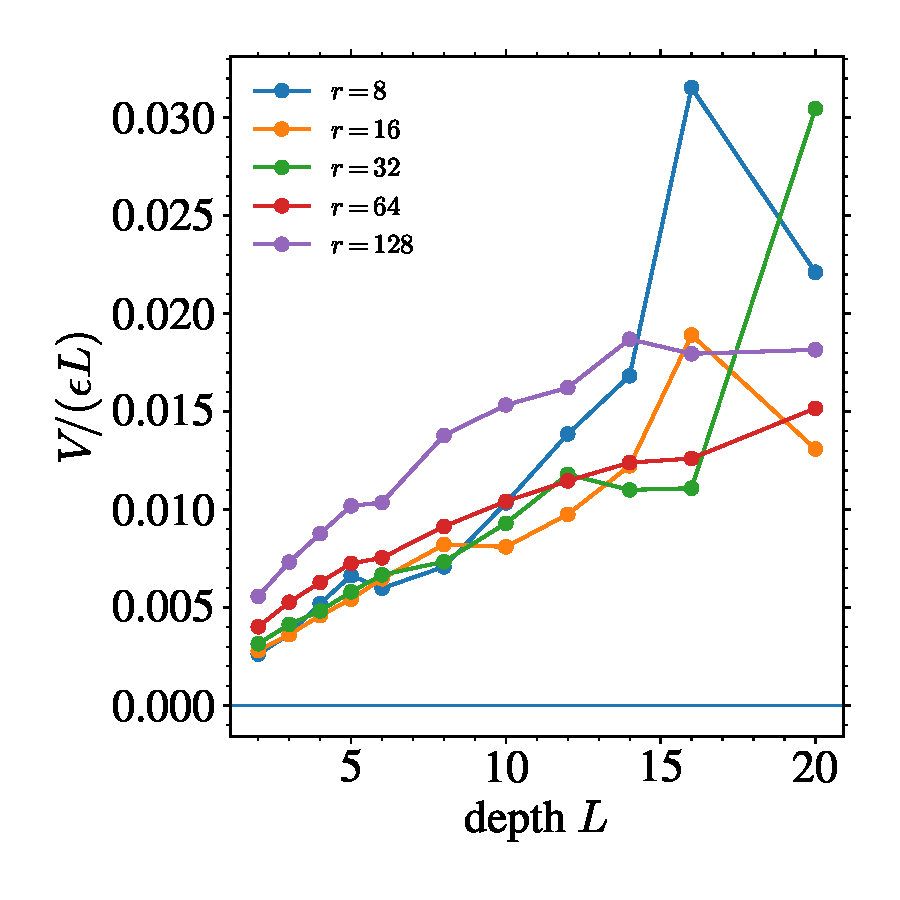
\includegraphics[width=\linewidth]{../../data/feynman/true_finite_ntk_cumulants_very_long/cumulant_ratio_V_same_off_over_eps_L.pdf}
\end{minipage}
\hfill
\begin{minipage}{0.32\linewidth}
\centering
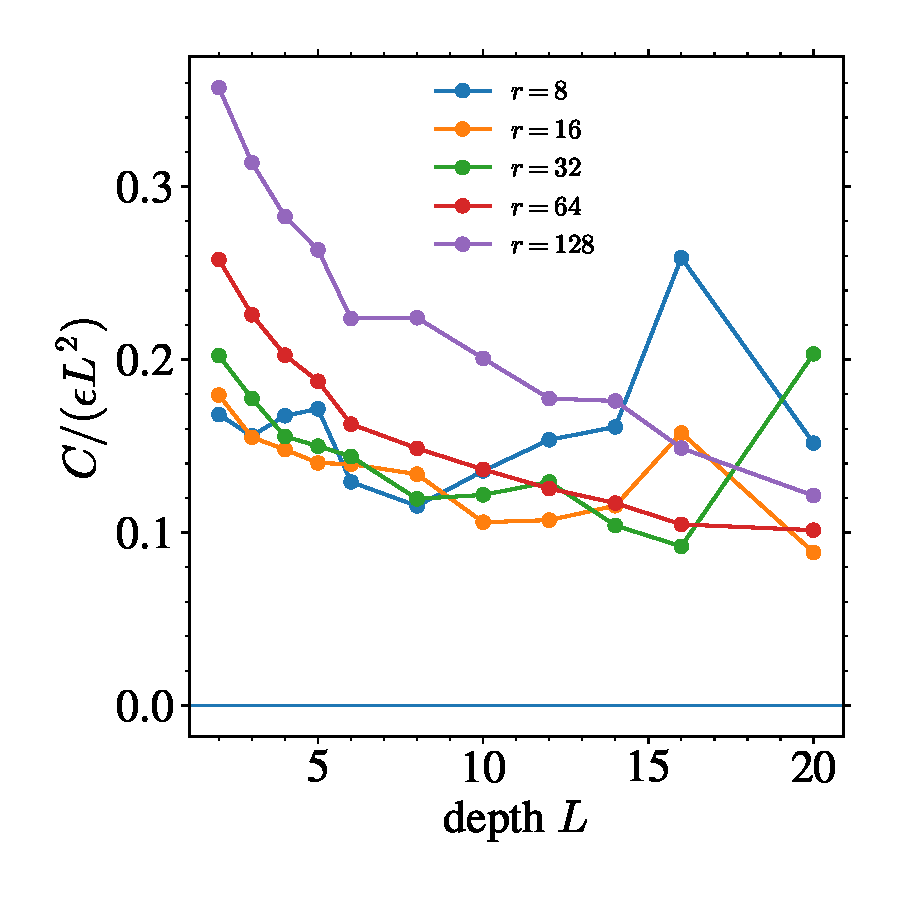
\includegraphics[width=\linewidth]{../../data/feynman/true_finite_ntk_cumulants_very_long/cumulant_ratio_C_same_off_over_eps_L2.pdf}
\end{minipage}
\hfill
\begin{minipage}{0.32\linewidth}
\centering
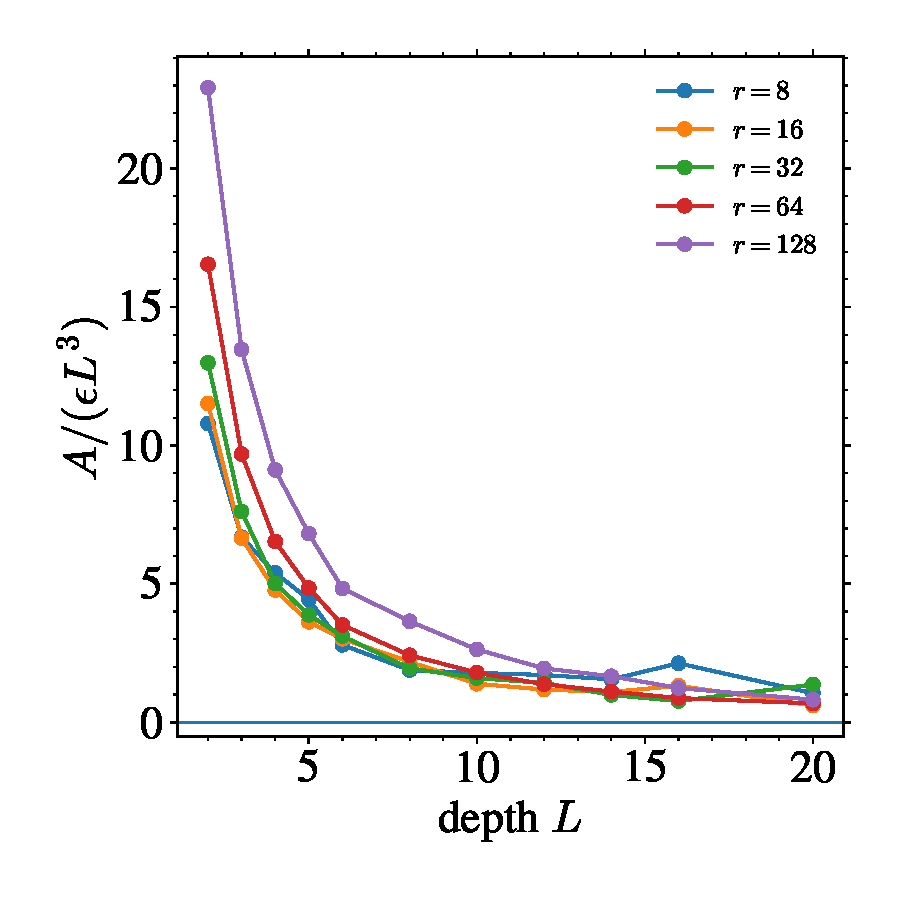
\includegraphics[width=\linewidth]{../../data/feynman/true_finite_ntk_cumulants_very_long/cumulant_ratio_A_same_off_over_eps_L3.pdf}
\end{minipage}
\caption{True finite-network cumulants from autodiff NTKs. These scalar-output cumulants are not isolated Feynman coefficients; they test the predicted polynomial control and rank-width scaling on actual finite networks.}
\label{fig:true-cumulants}
\end{figure}

\begin{table}[t]
\centering
\caption{Exact full-rank matching for true empirical NTKs at \(n=r=128\), \(m=8\), \(d=16\). Differences remain at numerical precision up to depth \(L=200\), confirming Theorem \ref{thm:pathwise}.}
\label{tab:full-rank-matching}
\begin{tabular}{ccc}
\toprule
Depth & max absolute NTK difference & relative difference \\
\midrule
2 & \(8.88\cdot10^{-16}\) & \(8.09\cdot10^{-17}\) \\
4 & \(3.55\cdot10^{-15}\) & \(1.31\cdot10^{-16}\) \\
6 & \(5.33\cdot10^{-15}\) & \(4.05\cdot10^{-16}\) \\
8 & \(3.55\cdot10^{-15}\) & \(4.20\cdot10^{-16}\) \\
10 & \(6.22\cdot10^{-15}\) & \(1.14\cdot10^{-15}\) \\
20 & \(1.95\cdot10^{-14}\) & \(3.77\cdot10^{-15}\) \\
50 & \(5.68\cdot10^{-14}\) & \(6.68\cdot10^{-16}\) \\
100 & \(2.14\cdot10^{-15}\) & \(2.35\cdot10^{-14}\) \\
200 & \(8.08\cdot10^{-14}\) & \(1.27\cdot10^{-14}\) \\
\bottomrule
\end{tabular}
\end{table}

\section{Conclusion}
Low rank changes finite-width NTK theory not only by reducing parameters, but by changing the stability threshold for training. In the unprojected RF-LR bottleneck, old NTK memory is geometrically shortened, but the centered spectral margin is also smaller. Combining these effects gives the main design message: preserving the NTK edge of convexity has a conservative cubic-depth sufficient rule, \(r\gtrsim mL^3\), up to logarithmic factors. A quadratic-depth rule is available only after the radial mode is projected out. The rank-width diagrammatics developed here connect these criteria to conditional operator concentration and to finite-network experiments.

The scope is deliberately narrow. The results apply to signed/isometric low-rank factors and RF-LR bottlenecks, not to strict positive NMF with cone constraints. The constants \(5\), \(21/20\), and \(173/720\) are isolated proxy/tensor constants, not direct scalar-output cumulant constants. The operator concentration theorem still keeps logarithmic factors and an explicit well-spread data distinction, and a full table of dNTK/ddNTK descendant coefficients remains future work.

\begin{thebibliography}{99}
\bibitem{Jacot2018}
A. Jacot, F. Gabriel, and C. Hongler.
\newblock Neural tangent kernel: convergence and generalization in neural networks.
\newblock \emph{NeurIPS}, 2018.

\bibitem{Lee2019}
J. Lee, L. Xiao, S. Schoenholz, Y. Bahri, J. Sohl-Dickstein, and J. Pennington.
\newblock Wide neural networks of any depth evolve as linear models under gradient descent.
\newblock \emph{NeurIPS}, 2019.

\bibitem{Du2019}
S. Du, J. Lee, H. Li, L. Wang, and X. Zhai.
\newblock Gradient descent finds global minima of deep neural networks.
\newblock \emph{ICML}, 2019.

\bibitem{AllenZhu2019}
Z. Allen-Zhu, Y. Li, and Z. Song.
\newblock A convergence theory for deep learning via over-parameterization.
\newblock \emph{ICML}, 2019.

\bibitem{Arora2019}
S. Arora, S. Du, W. Hu, Z. Li, R. Salakhutdinov, and R. Wang.
\newblock On exact computation with an infinitely wide neural net.
\newblock \emph{NeurIPS}, 2019.

\bibitem{NguyenMondelli2020}
Q. Nguyen and M. Mondelli.
\newblock Global convergence of deep networks with one wide layer followed by pyramidal topology.
\newblock arXiv:2002.07867, 2020.

\bibitem{NguyenMondelliMontufar2022}
Q. Nguyen, M. Mondelli, and G. Montúfar.
\newblock Tight bounds on the smallest eigenvalue of the neural tangent kernel for deep ReLU networks.
\newblock arXiv:2012.11654, 2020/2022.

\bibitem{Yang2019}
G. Yang.
\newblock Wide feedforward or recurrent neural networks of any architecture are Gaussian processes.
\newblock \emph{NeurIPS}, 2019.

\bibitem{Yang2021}
G. Yang and E. Hu.
\newblock Tensor programs IV: Feature learning in infinite-width neural networks.
\newblock \emph{ICML}, 2021.

\bibitem{Huang2020}
J. Huang and H.-T. Yau.
\newblock Dynamics of deep neural networks and neural tangent hierarchy.
\newblock \emph{ICML}, 2020.

\bibitem{DyerGurAri2019}
E. Dyer and G. Gur-Ari.
\newblock Asymptotics of wide networks from Feynman diagrams.
\newblock arXiv:1909.11304, 2019.

\bibitem{FeynmanNTK2026}
M. Guillen, P. Misof, and J. E. Gerken.
\newblock Finite-width neural tangent kernels from Feynman diagrams.
\newblock arXiv:2508.11522, 2025/2026.

\bibitem{RFLR2026}
Anonymous authors.
\newblock Low rank is enough for the neural tangent kernel: towards stable training of deep networks.

\bibitem{Novak2022}
R. Novak, J. Sohl-Dickstein, and S. Schoenholz.
\newblock Fast finite width neural tangent kernel.
\newblock \emph{ICML}, 2022.

\bibitem{Zeng2024LoRA}
Y. Zeng and collaborators.
\newblock LoRA training in the NTK regime has no spurious local minima.
\newblock arXiv:2402.11867, 2024.

\bibitem{MosigGarciaAgazziTrevisan2025}
E. Mosig García, A. Agazzi, and D. Trevisan.
\newblock Quantitative convergence of trained single layer neural networks to Gaussian processes.
\newblock arXiv:2509.24544, 2025.
\end{thebibliography}

\appendix

\section{Full Proof of the Frozen-Left Decomposition}
\label{app:frozen-left-full-proof}
We prove Proposition \ref{prop:frozen-left}. Consider one layer
\[
W=\alpha UB,\qquad U^\top U=I_r,\qquad B\in\R^{r\times d},
\]
and let \(H=\partial \mathcal L/\partial W\) be the Euclidean loss gradient in dense-weight coordinates. The Frobenius inner product is used throughout.

First freeze \(U\). For a variation \(dB\),
\[
dW=\alpha U\,dB,
\qquad
d\mathcal L
=\langle H,\alpha U\,dB\rangle
=\langle \alpha U^\top H,dB\rangle.
\]
Hence \(\nabla_B\mathcal L=\alpha U^\top H\). Gradient descent in \(B\) gives
\[
\dot B=-\eta\alpha U^\top H,
\qquad
\dot W_B=\alpha U\dot B
=-\eta\alpha^2UU^\top H,
\]
which is \eqref{eq:frozen-left-flow}. Therefore the \(B\)-only tangent directions are exactly the fixed linear subspace
\[
\mathcal T_B W=\{\alpha U\Delta B:\Delta B\in\R^{r\times d}\}.
\]
The corresponding contribution to the empirical NTK is a fixed-projector block, because every dense gradient is projected through \(UU^\top\).

Now allow \(U\) to vary on the Stiefel manifold \(\mathrm{St}(n,r)=\{U:U^\top U=I_r\}\). Its tangent space is
\[
T_U\mathrm{St}(n,r)
=\{\Delta U:U^\top\Delta U+\Delta U^\top U=0\}.
\]
Every tangent vector decomposes as
\[
\Delta U=U\Omega+U_\perp K,
\qquad
\Omega^\top=-\Omega,
\qquad
U^\top U_\perp=0,
\]
where \(U\Omega\) rotates the basis inside \(\operatorname{span}(U)\) and \(U_\perp K=(I-UU^\top)\Delta U\) moves the subspace itself. For a variation \(dU\),
\[
dW=\alpha\,dU\,B,
\qquad
d\mathcal L
=\langle H,\alpha dU B\rangle
=\langle \alpha H B^\top,dU\rangle.
\]
Thus the Euclidean gradient in \(U\)-coordinates is \(\alpha HB^\top\). Its normal subspace-moving component is
\[
(I-UU^\top)\alpha HB^\top.
\]
The skew component \(U\Omega\) only rotates coordinates inside the same represented subspace: by replacing \(U\) with \(UR\) and \(B\) with \(R^\top B\), the product \(UB\) is unchanged. This is why the main text states \eqref{eq:moving-left-flow} up to rotations inside \(\operatorname{span}(U)\) that can be absorbed into \(B\).

Keeping only the subspace-moving component, Stiefel gradient descent contributes
\[
\dot U_{\perp}
=-\eta\alpha(I-UU^\top)HB^\top.
\]
Mapping this velocity back to dense-weight coordinates gives
\[
\dot W_U
=\alpha \dot U_{\perp}B
=-\eta\alpha^2(I-UU^\top)H B^\top B,
\]
which is \eqref{eq:moving-left-flow}. This term is absent when \(U\) is frozen. It depends on the current right factor through \(B^\top B\), so it cannot be represented by cumulants of the fixed Haar projector \(G=(n/r)UU^\top\) alone.

Finally, if both \(U\) and \(B\) are trained, the tangent space contains the sum of \(B\)-directions \(\alpha U\Delta B\), Stiefel subspace directions \(\alpha\Delta U B\), and their cross terms in the NTK Gram matrix. Along gradient flow these directions also vary in time, producing dNTK terms involving \(\dot U\), \(\dot B\), and products such as \(B^\top B\). The frozen-left model deliberately removes these moving-subspace interactions, leaving a closed fixed-projector diagrammatic calculus.

\section{Projector Cumulants Beyond Second Order}
For \(G=(n/r)UU^\top\), the mean is \(\E G=I_n\), the trace is deterministic, and every connected cumulant containing the trace direction vanishes. Orthogonal Weingarten calculus gives, for fixed cumulant order \(s\),
\begin{equation}
\cumul(G_{i_1j_1},\ldots,G_{i_sj_s})
=O_s(r^{1-s})
\end{equation}
uniformly when \(r\le n\) and \(r\to\infty\), with the full-rank endpoint cancelling after replacing \(r^{-1}\) by the defect scale \(\gamma_{n,r}\) at second order. Diagrammatically, this is why a connected rank vertex is counted by the number of connected projector insertions, not simply by the number of factors \(U\) in the algebraic expression.

\section{Low-Rank Diagrammatic Rules}
\label{app:diagrammatic-rules}
This appendix records the graphical calculus underlying the perturbative statements in the main text. The external objects are the same as in finite-width NTK Feynman diagrams: NNGP/preactivation legs, NTK fluctuation legs, and derivative-NTK descendants. The difference is internal. In the low-rank model, stochastic vertices are empirical rank cumulants and frozen-projector cumulants rather than unconstrained neural-index contractions.

\subsection{Visual dictionary}
We use the same visual grammar as the finite-width NTK diagrammatics: filled external dots denote observed sample indices, solid lines denote NNGP/preactivation objects, colored dotted ghost lines denote NTK fluctuations, and multi-line ghost objects denote dNTK/ddNTK descendants. Low-rank only changes the internal stochastic vertices.
\begin{align}
z_\alpha
&\equiv
\begin{tikzpicture}[baseline=-0.1cm]
  \begin{feynman}
    \vertex[right=0pt, dot, minimum size=3pt, label={left:{\footnotesize \(\alpha\)}}] (x) {};
    \vertex[right=30pt of x, dot, minimum size=0pt] (b) {};
    \diagram*{(x) -- [inner sep=4pt] (b)};
  \end{feynman}
\end{tikzpicture}
\qquad
\widehat{\Delta\Theta}_{\textcolor{color1}{\alpha\beta}}
\equiv
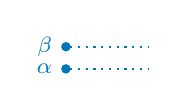
\begin{tikzpicture}[baseline=0.05cm]
  \begin{feynman}
    \vertex[color1, dot, minimum size=3pt, label={left:{\footnotesize \(\textcolor{color1}{\alpha}\)}}] (x1) {};
    \vertex[above=8pt of x1, color1, dot, minimum size=3pt, label={left:{\footnotesize \(\textcolor{color1}{\beta}\)}}] (x2) {};
    \vertex[right=30pt of x1, dot, minimum size=0pt] (b1) {};
    \vertex[right=30pt of x2, dot, minimum size=0pt] (b2) {};
    \diagram*{
      (x1) -- [color1, ghost, inner sep=4pt] (b1),
      (x2) -- [color1, ghost, inner sep=4pt] (b2)
    };
  \end{feynman}
\end{tikzpicture}
\qquad
\widehat{\mathrm d\Theta}
\equiv
\begin{tikzpicture}[baseline=0.05cm]
  \begin{feynman}
    \vertex[color3, dot, minimum size=3pt] (x0) {};
    \vertex[above=8pt of x0, color1, dot, minimum size=3pt] (x1) {};
    \vertex[above=8pt of x1, color6, dot, minimum size=3pt] (x2) {};
    \vertex[right=30pt of x0, dot, minimum size=0pt] (b0) {};
    \vertex[right=30pt of x1, dot, minimum size=0pt] (b1) {};
    \vertex[right=30pt of x2, dot, minimum size=0pt] (b2) {};
    \diagram*{
      (x0) -- [color6color1ddntknew, inner sep=4pt] (b0),
      (x1) -- [color1, ghost, inner sep=4pt] (b1),
      (x2) -- [color6, ghost, inner sep=4pt] (b2)
    };
  \end{feynman}
\end{tikzpicture}.
\label{eq:appendix-visual-external}
\end{align}
The new internal low-rank vertices are:
\begin{align}
\text{rank cumulant}
&\equiv
\begin{tikzpicture}[baseline=(r)]
  \begin{feynman}
    \vertex[rankblob] (r) {\scriptsize \(\kappa_s\)};
    \vertex[left=25pt of r, dot, minimum size=0pt] (l) {};
    \vertex[above right=18pt and 25pt of r, dot, minimum size=0pt] (u) {};
    \vertex[right=25pt of r, dot, minimum size=0pt] (rr) {};
    \vertex[below right=18pt and 25pt of r, dot, minimum size=0pt] (d) {};
    \diagram*{
      (l) -- [color2, ghost] (r),
      (u) -- [color2, ghost] (r),
      (rr) -- [color2, ghost] (r),
      (d) -- [color2, ghost] (r)
    };
  \end{feynman}
\end{tikzpicture}
\sim r^{1-s}\kappa_s,
\qquad
\text{projector cumulant}
\equiv
\begin{tikzpicture}[baseline=(h)]
  \begin{feynman}
    \vertex[haarblob] (h) {\scriptsize \(G\)};
    \vertex[left=26pt of h, dot, minimum size=0pt] (l) {};
    \vertex[above right=16pt and 26pt of h, dot, minimum size=0pt] (u) {};
    \vertex[below right=16pt and 26pt of h, dot, minimum size=0pt] (d) {};
    \diagram*{
      (l) -- [color4, photon] (h),
      (u) -- [color4, photon] (h),
      (d) -- [color4, photon] (h)
    };
  \end{feynman}
\end{tikzpicture}
\sim \cumul(G,\ldots,G).
\label{eq:appendix-visual-lowrank}
\end{align}

\subsection{Rank-state vertices}
Let
\begin{equation}
M_A^{(\ell)}
=\frac1{r_\ell}\sum_{a=1}^{r_\ell}\phi_A^{(\ell)}(Z_a),
\label{eq:appendix-rank-state}
\end{equation}
where \(A\) labels a local atom such as \(\sigma\sigma\), \(\sigma\sigma'\), \(\sigma'\sigma'\), or a derivative analogue. Conditional on the past, the rank atoms are iid. Therefore
\(Z_a\) is the same channel-local random object defined in Lemma \ref{lem:rank-cumulant-counting}, with the layer superscript suppressed.
\begin{equation}
\cumul(M_{A_1}^{(\ell)},\ldots,M_{A_s}^{(\ell)})
=r_\ell^{1-s}\kappa_{A_1\cdots A_s}^{(\ell)},
\qquad
\kappa_{A_1\cdots A_s}^{(\ell)}
=\cumul(\phi_{A_1}^{(\ell)}(Z),\ldots,\phi_{A_s}^{(\ell)}(Z)).
\label{eq:appendix-rank-vertex}
\end{equation}
Thus every connected rank vertex of valence \(s\) has weight \(r_\ell^{1-s}\). In the isometric model, one also has frozen-projector vertices given by cumulants of \(G=(n/r)UU^\top\). At valence two this is Lemma \ref{lem:haar-cov}; at higher valence the weights are orthogonal Weingarten contractions. When \(r=n\), \(G=I\), so every centered projector vertex vanishes.

\begin{theorem}[Low-rank Feynman rules]
\label{thm:lowrank-feynman-rules}
Let \(F\) be a smooth observable of finitely many layer states \(M^{(\ell)}\) and frozen projectors \(G^{(\ell)}\). Its expansion in powers of \(1/r_\ell\) and projector cumulants is obtained by summing connected low-rank diagrams with the prescribed external legs. Algebraically:
\begin{enumerate}[leftmargin=1.5em]
\item a rank vertex of valence \(s\) contributes \(r_\ell^{1-s}\kappa_s^{(\ell)}\);
\item a projector vertex contributes the corresponding cumulant of \(G^{(\ell)}\), with second-order scale \(\gamma_{n_\ell,r_\ell}\);
\item a deterministic layer vertex contributes a Frechet derivative \(D^q\Phi_\ell\) of the layer map;
\item a transport edge contributes the product of first derivatives along the depth path;
\item for cumulants, disconnected diagrams cancel by the moment-cumulant relation.
\end{enumerate}
\end{theorem}

\begin{proof}
Taylor expand \(F\) around the deterministic trajectory of the rank states. The cumulant generating operator for an empirical rank average is
\begin{equation}
\exp\left(
\sum_{s\ge2}\frac{r^{1-s}}{s!}
\kappa_{A_1\cdots A_s}
\partial_{A_1}\cdots\partial_{A_s}
\right),
\label{eq:appendix-edgeworth}
\end{equation}
up to the usual finite-order smoothness remainder. Expanding \eqref{eq:appendix-edgeworth} gives the rank vertices and their deterministic derivative contractions. The same argument applies to \(G\), replacing empirical-rank cumulants by frozen-projector cumulants. Taking connected cumulants removes disconnected products.
\end{proof}

\subsection{Basic tensor recursions}
The diagrammatic rules produce the same external tensor hierarchy as the dense finite-width expansion, but with low-rank sources. Let \(J^K_\ell\) and \(J^\Theta_\ell\) denote the deterministic linear transports for NNGP and NTK legs. The NNGP covariance block satisfies schematically
\begin{equation}
V_{\ell+1}
=J^K_\ell V_\ell (J^K_\ell)^\top+\Xi^{KK}_\ell,
\qquad
\Xi^{KK}_\ell
=r_\ell^{-1}\kappa_2(S^K,S^K)
+\gamma_{n_\ell,r_\ell}\mathfrak h^{KK}_\ell.
\label{eq:appendix-V-rec}
\end{equation}
For the mixed NNGP-NTK block \(C=(D,F)\),
\begin{equation}
C_{\ell+1}
=J^K_\ell C_\ell (J^\Theta_\ell)^\top
+\mathsf S_V[V_\ell]
+\Xi^{K\Theta}_\ell.
\label{eq:appendix-C-rec}
\end{equation}
For the NTK-NTK block \(A=(A,B)\),
\begin{equation}
A_{\ell+1}
=J^\Theta_\ell A_\ell (J^\Theta_\ell)^\top
+\mathsf S_C[C_\ell]+\mathsf S_V[V_\ell]
+\Xi^{\Theta\Theta}_\ell.
\label{eq:appendix-A-rec}
\end{equation}
The sources \(\Xi^{KK}\), \(\Xi^{K\Theta}\), and \(\Xi^{\Theta\Theta}\) are precisely the rank and projector cumulant vertices with the corresponding external legs. This explains why the depth exponents in Proposition \ref{prop:tensor-hierarchy} come from external transport, while the small parameters come from \(r^{-1}\), \(1/n\), and \(\gamma_{n,r}\).
\begin{equation}
\begin{tikzpicture}[baseline=(vbase)]
  \begin{feynman}
    \vertex (vbase) at (0,0) {};
    \vertex[dot, minimum size=3pt] (k1) at (0,0.45) {};
    \vertex[dot, minimum size=3pt] (k2) at (0,-0.45) {};
    \vertex[quarticblob] (v) at (1.6,0) {\scriptsize \(V\)};
    \vertex[rankblob] (rv) at (3.3,0) {\scriptsize \(\kappa_2\)};
    \diagram*{
      (k1) -- (v) -- (k2),
      (v) -- [color2, ghost, edge label={\scriptsize source}] (rv)
    };
  \end{feynman}
\end{tikzpicture}
\qquad
\begin{tikzpicture}[baseline=(cbase)]
  \begin{feynman}
    \vertex (cbase) at (0,0) {};
    \vertex[dot, minimum size=3pt] (k) at (0,0.45) {};
    \vertex[color1, dot, minimum size=3pt] (t) at (0,-0.45) {};
    \vertex[quarticblob] (c) at (1.6,0) {\scriptsize \(C\)};
    \vertex[rankblob] (rc) at (3.3,0) {\scriptsize \(\kappa_2\)};
    \diagram*{
      (k) -- (c),
      (t) -- [color1, ghost] (c),
      (c) -- [color2, ghost, edge label={\scriptsize source}] (rc)
    };
  \end{feynman}
\end{tikzpicture}
\qquad
\begin{tikzpicture}[baseline=(abase)]
  \begin{feynman}
    \vertex (abase) at (0,0) {};
    \vertex[color1, dot, minimum size=3pt] (t1) at (0,0.45) {};
    \vertex[color2, dot, minimum size=3pt] (t2) at (0,-0.45) {};
    \vertex[quarticblob] (a) at (1.6,0) {\scriptsize \(A\)};
    \vertex[rankblob] (ra) at (3.3,0) {\scriptsize \(\kappa_2\)};
    \diagram*{
      (t1) -- [color1, ghost] (a),
      (t2) -- [color2, ghost] (a),
      (a) -- [color2, ghost, edge label={\scriptsize source}] (ra)
    };
  \end{feynman}
\end{tikzpicture}
\label{eq:appendix-visual-VCA}
\end{equation}

\subsection{First NTK mean correction}
The familiar finite-width correction to the NTK mean has the same external five-term form:
\begin{equation}
\Theta^{\{1\}}_{\ell+1}
=\mathsf T_\Theta[\Theta^{\{1\}}_\ell]
+\mathsf T_K[K^{\{1\}}_\ell]
+\mathsf S_V[V_\ell]
+\mathsf S_D[D_\ell]
+\mathsf S_F[F_\ell].
\label{eq:appendix-theta-five}
\end{equation}
The low-rank difference is that the source tensors \(V,D,F\) are further resolved into the rank-state and projector vertices above. Thus the low-rank calculus does not change the external NTK grammar; it changes the internal expansion parameter from neural-index contractions to empirical-rank cumulants and frozen-projector cumulants.

\subsection{Pairing extraction}
A rank-four orthogonally invariant tensor decomposes as
\begin{equation}
C_{i_1i_2i_3i_4}
=c_1\delta_{i_1i_2}\delta_{i_3i_4}
+c_2\delta_{i_1i_3}\delta_{i_2i_4}
+c_3\delta_{i_1i_4}\delta_{i_2i_3}.
\label{eq:appendix-pairing}
\end{equation}
Let \(B_1,B_2,B_3\) be the three pairings. The normalized pairing Gram matrix is
\begin{equation}
\overline G_N
=
\begin{pmatrix}
1&1/N&1/N\\
1/N&1&1/N\\
1/N&1/N&1
\end{pmatrix},
\qquad
\overline G_N^{-1}
=\frac{N}{N-1}I_3-\frac{N}{(N-1)(N+2)}\one\one^\top.
\label{eq:appendix-pairing-inv}
\end{equation}
If \(h=(\langle C,B_1\rangle,\langle C,B_2\rangle,\langle C,B_3\rangle)\) are measured contractions, the isolated tensor coefficients are \((c_1,c_2,c_3)^\top=\overline G_N^{-1}h\). This is why direct scalar-output cumulants should not be identified with the endpoint coefficients \(5\), \(21/20\), and \(173/720\) without a pairing-basis extraction.

\subsection{Centered RF-LR memory lemma}
For RF-LR, an old NTK line transported from layer \(k\) to \(L\) carries
\begin{equation}
B_{L:k}
=\prod_{s=k+1}^{L}\frac1r\dot\Sigma^{(s)}.
\label{eq:appendix-rflr-product}
\end{equation}
At ReLU edge of chaos, \(\dot\Sigma^{(s)}\to1/2\), so \(\|B_{L:k}\|\lesssim (2r)^{-(L-k)}\), up to polynomial endpoint factors. The corresponding centered transport diagram is
\begin{equation}
\begin{tikzpicture}[baseline=(y)]
  \begin{feynman}
    \vertex[projblob] (p1) at (0,0) {\scriptsize \(P\)};
    \vertex[rankblob] (y) at (1.1,0) {\scriptsize \(Y_k\)};
    \vertex[smallblob] (b1) at (2.3,0) {};
    \vertex (dots) at (3.0,0) {\(\cdots\)};
    \vertex[smallblob] (b2) at (3.8,0) {};
    \vertex[projblob] (p2) at (5.0,0) {\scriptsize \(P\)};
    \diagram*{
      (p1) -- [color1, ghost] (y) -- [color1, ghost, edge label={\scriptsize \(b\simeq(2r)^{-1}\)}] (b1),
      (b2) -- [color1, ghost] (p2)
    };
    \draw[color1,dash pattern=on 3pt off 3pt,line width=1pt] (b1) -- (dots);
    \draw[color1,dash pattern=on 3pt off 3pt,line width=1pt] (dots) -- (b2);
  \end{feynman}
\end{tikzpicture}
\label{eq:appendix-visual-centered-memory}
\end{equation}
Let \(P=I-\one\one^\top/m\) and \(Z_L=P(\widehat K_L-K_L)P\). The centered fluctuation admits the linearized expansion
\begin{equation}
Z_L
=\sum_{k=1}^{L}B_{L:k+1}Y_k
+\sum_{k=1}^{L}B_{L:k+1}R_k,
\label{eq:appendix-centered-expansion}
\end{equation}
where \(Y_k\) is a centered fresh rank source and \(R_k\) is quadratic in earlier fluctuations.

\begin{lemma}[Centered RF-LR memory]
\label{lem:centered-rflr-memory}
Assume, conditionally on the past,
\begin{equation}
\left\|\E[Y_k^2\mid\mathcal F_{k-1}]\right\|_{\op}
\le C\frac{m\eps_{\RF}}{r^2},
\qquad
\|Y_k\|_{\psi_1}\le C\frac{\sqrt{\eps_{\RF}}}{r},
\label{eq:appendix-Y-bound}
\end{equation}
and \(\|B_{L:k}\|\le q^{L-k}\) for some \(q<1\). If \(\|R_k\|_{\op}\le C m\eps_{\RF}/r^2\) with high probability, then, up to logarithmic factors,
\begin{equation}
\|Z_L\|_{\op}
\lesssim
\frac{\sqrt{m\eps_{\RF}\log(m/\delta)}}{r}
+
\frac{m\eps_{\RF}\log(m/\delta)}{r^2}
\label{eq:appendix-centered-lemma}
\end{equation}
with probability at least \(1-\delta\).
\end{lemma}

\begin{proof}
Set \(X_k=B_{L:k+1}Y_k\). The predictable matrix variance satisfies
\begin{equation}
\left\|\sum_{k=1}^{L}\E[X_k^2\mid\mathcal F_{k-1}]\right\|_{\op}
\le
C\frac{m\eps_{\RF}}{r^2}\sum_{k=1}^{L}q^{2(L-k)}
\le C'\frac{m\eps_{\RF}}{r^2}.
\end{equation}
Matrix Freedman or Bernstein gives the first term in \eqref{eq:appendix-centered-lemma}. For the quadratic remainder,
\begin{equation}
\left\|\sum_{k=1}^{L}B_{L:k+1}R_k\right\|_{\op}
\le
C\frac{m\eps_{\RF}}{r^2}\sum_{k=1}^{L}q^{L-k}
\le C'\frac{m\eps_{\RF}}{r^2}.
\end{equation}
\end{proof}

Combining Lemma \ref{lem:centered-rflr-memory} with Weyl's inequality gives the centered/angularized criterion. If the centered deterministic margin satisfies \(\lambda_{\min}(PK_LP)\gtrsim (rL)^{-1}\), and if \(\eps_{\RF}\simeq 1/r\), then the fluctuation bound is below the margin when
\begin{equation}
r\gtrsim mL^2
\label{eq:appendix-centered-L2}
\end{equation}
up to logarithms. Without removing the radial constant mode, a diffusive \(\sqrt L\) factor can reappear, giving the conservative cubic-depth criterion used for the unprojected RF-LR statement.

\section{Why Strict Positive NMF Is Not Covered}
The model in \eqref{eq:intro-model} is signed and isometric. The right factor \(B\) is unconstrained and the frozen left factor \(U\) has orthonormal columns. Strict nonnegative matrix factorization imposes a cone constraint and changes the tangent space even at initialization. Its NTK is a projected or conic kernel, not the fixed linear-subspace kernel analyzed here. Therefore the results should not be cited as a theorem for positive NMF without a separate analysis of active constraints, boundary faces, and cone-projected gradients.

\section{Proof Details for Endpoint Constants}
For \(g\sim\mathcal N(0,1)\), let \(X_0=2(g_+)^2\) and \(Y_0=2\one_{\{g>0\}}\). Since \(\E[g_+^2]=1/2\) and \(\E[g_+^4]=3/2\), we have \(\E X_0=1\), \(\E X_0^2=6\), and \(\Var(X_0)=5\). Also \(\E Y_0=1\), \(\E Y_0^2=2\), so \(\Var(Y_0)=1\). Finally, \(\E X_0Y_0=2\), hence \(\Cov(X_0,Y_0)=1\). Transporting one or two NTK legs and applying the ReLU edge-of-chaos transport sum gives the formulas for \(B_\lambda\) and \(A_{\lambda,\mu}\).

\section{Additional Experimental Figures}

\begin{figure}[h]
\centering
\begin{minipage}{0.32\linewidth}
\centering
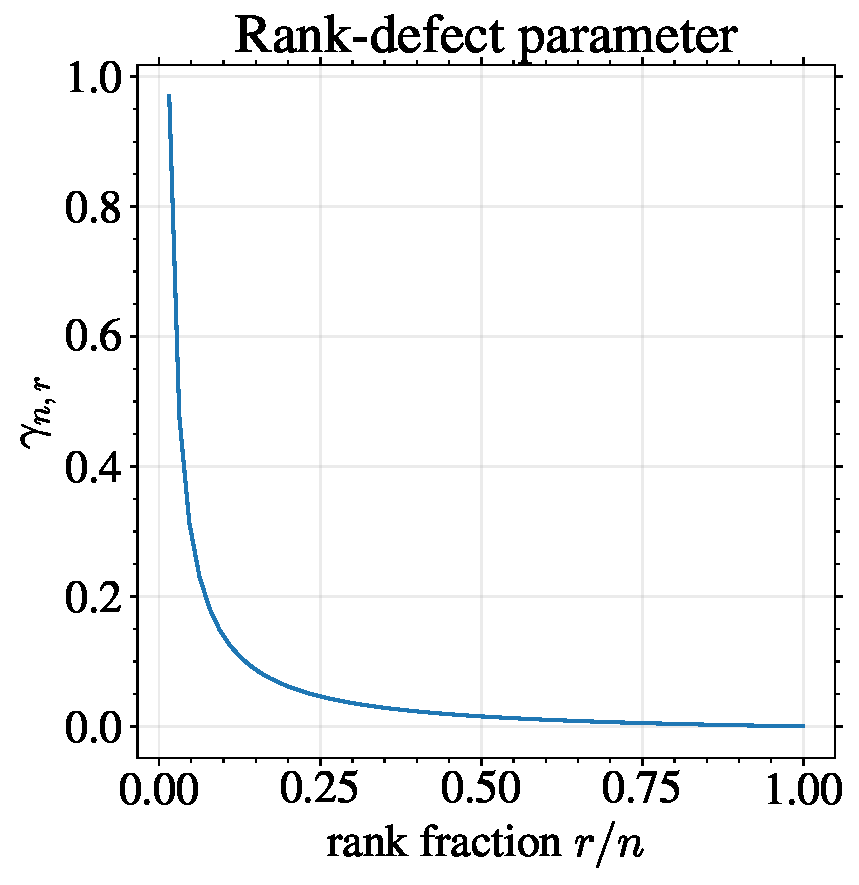
\includegraphics[width=\linewidth]{../../data/feynman/lowrank_ntk_proxy_outputs_clean/rank_defect_gamma.pdf}
\end{minipage}
\hfill
\begin{minipage}{0.32\linewidth}
\centering
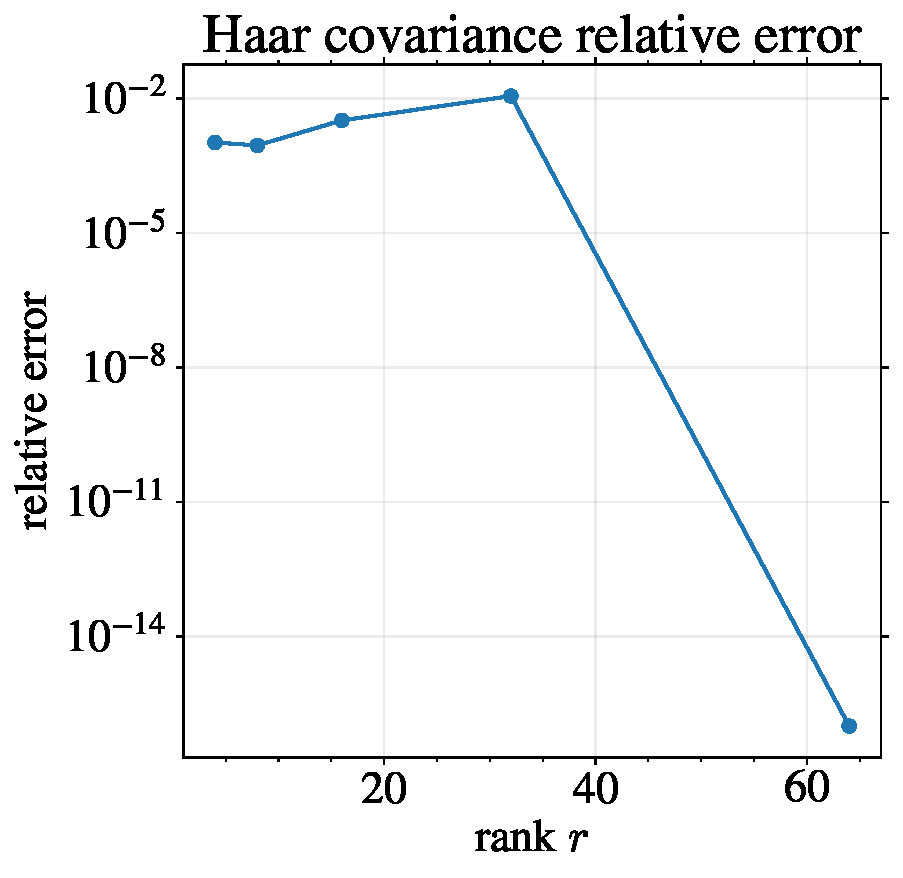
\includegraphics[width=\linewidth]{../../data/feynman/lowrank_ntk_proxy_outputs_clean/haar_covariance_relative_error.pdf}
\end{minipage}
\hfill
\begin{minipage}{0.32\linewidth}
\centering
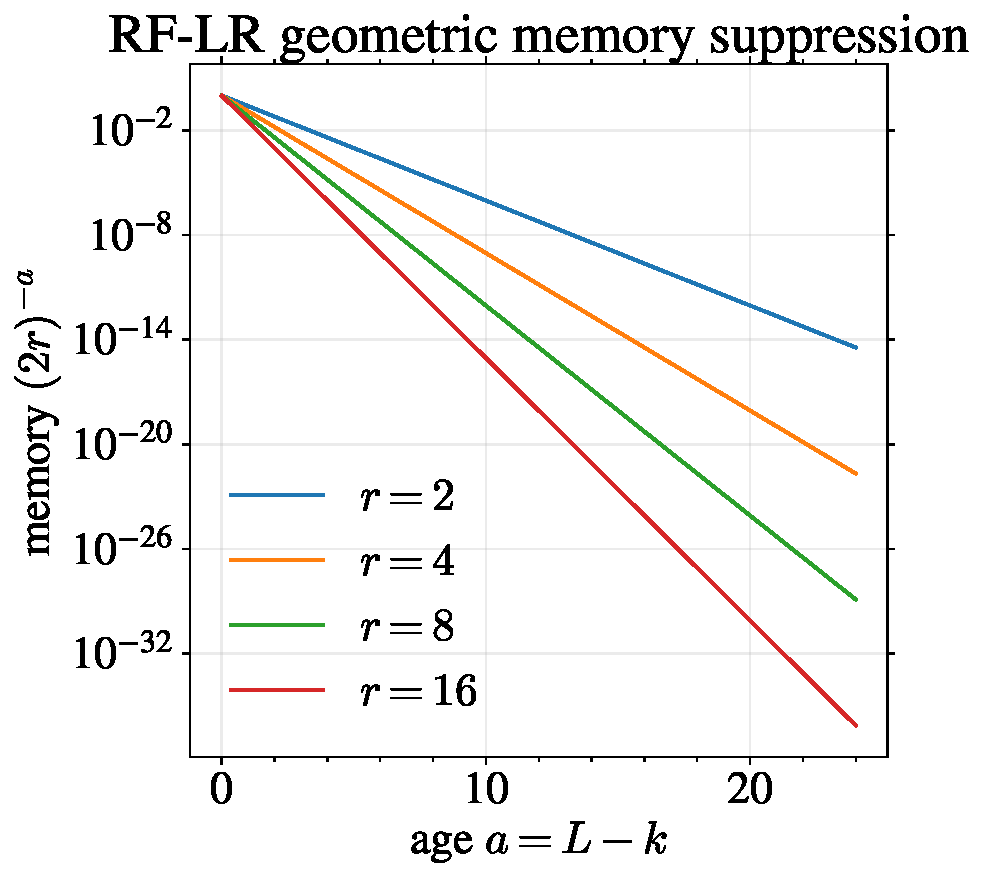
\includegraphics[width=\linewidth]{../../data/feynman/lowrank_ntk_proxy_outputs_clean/rflr_memory_suppression.pdf}
\end{minipage}
\caption{Additional proxy diagnostics: rank-defect parameter, relative Haar covariance error, and RF-LR geometric memory suppression.}
\label{fig:appendix-proxy-extra}
\end{figure}

\begin{figure}[h]
\centering
\begin{minipage}{0.32\linewidth}
\centering
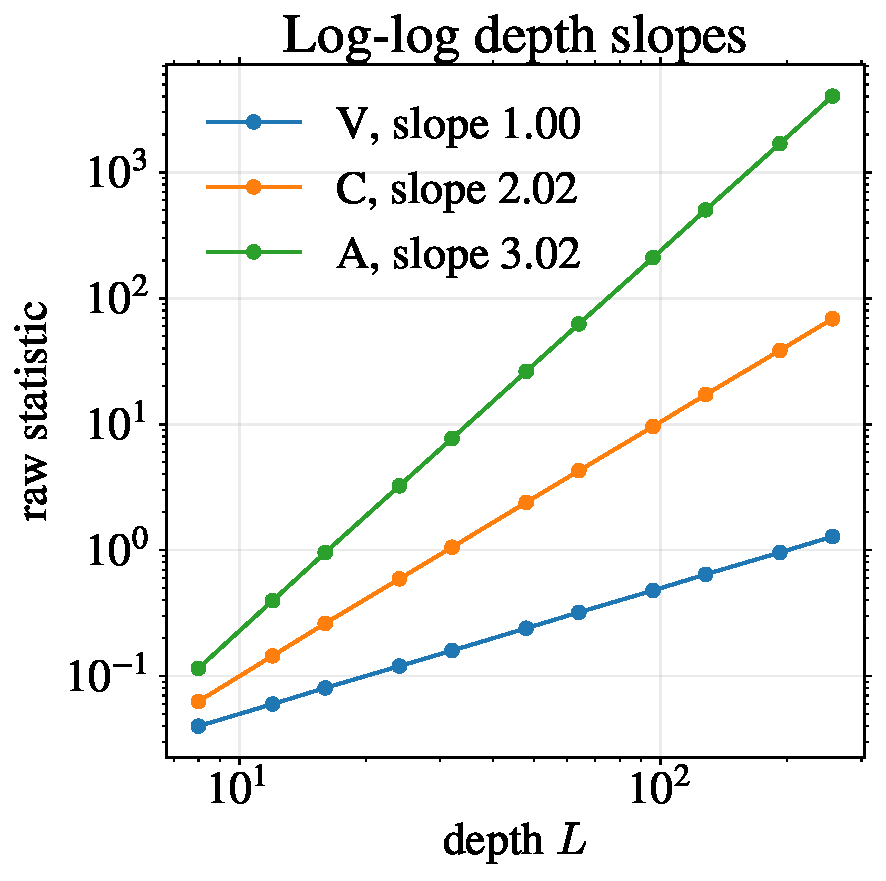
\includegraphics[width=\linewidth]{../../data/feynman/lowrank_ntk_proxy_outputs_clean/loglog_slopes_scalar_modes.pdf}
\end{minipage}
\hfill
\begin{minipage}{0.32\linewidth}
\centering
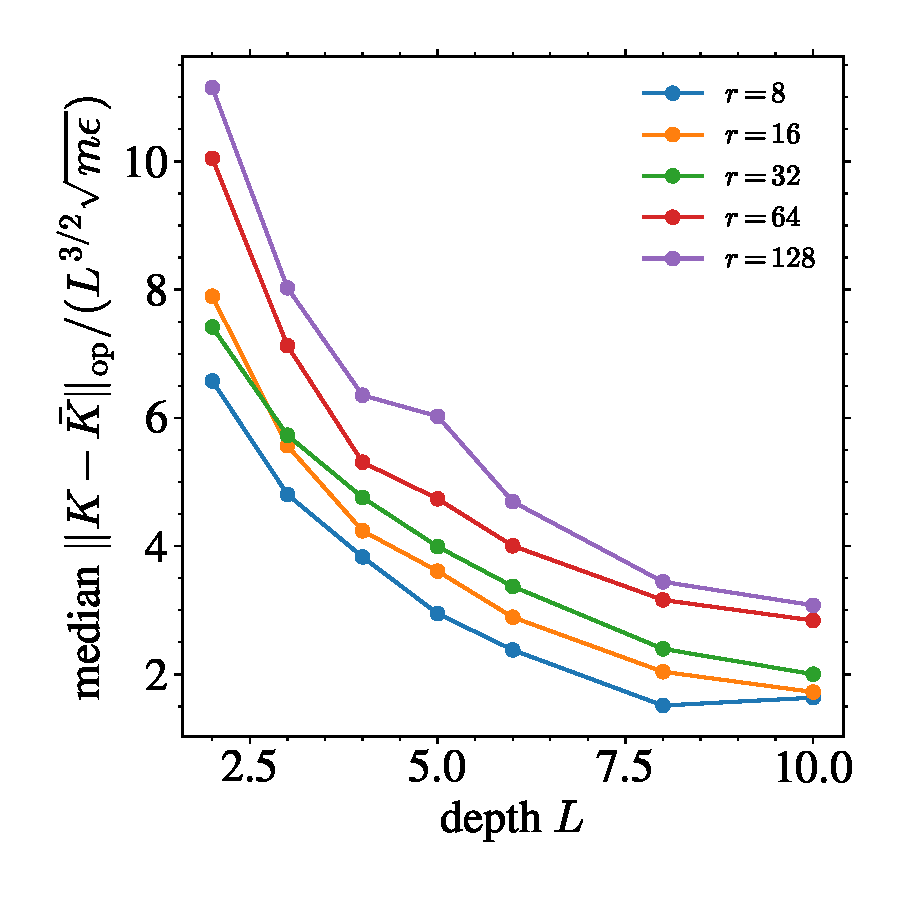
\includegraphics[width=\linewidth]{../../data/feynman/true_finite_ntk_outputs_clean/true_finite_ntk_operator_ratio.pdf}
\end{minipage}
\hfill
\begin{minipage}{0.32\linewidth}
\centering
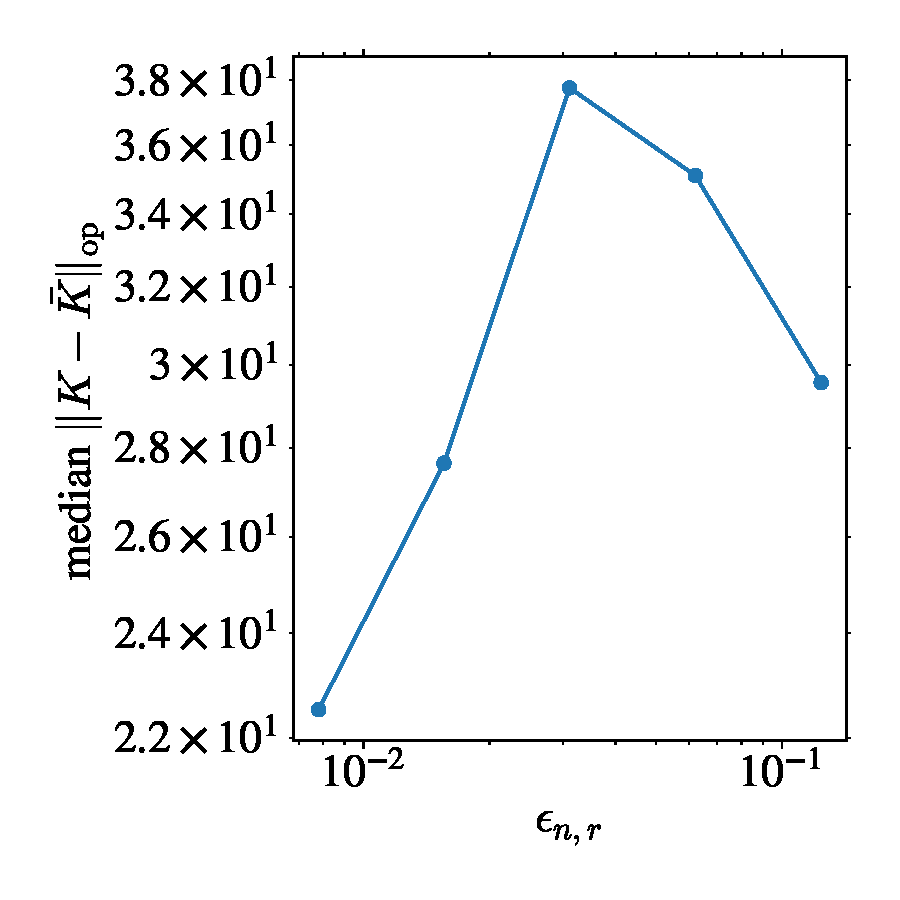
\includegraphics[width=\linewidth]{../../data/feynman/true_finite_ntk_outputs_clean/true_finite_ntk_rank_defect_scaling.pdf}
\end{minipage}
\caption{Depth-slope proxy diagnostics and true finite-network NTK operator/rank-defect checks.}
\label{fig:appendix-true-ntk}
\end{figure}

\begin{figure}[h]
\centering
\begin{minipage}{0.32\linewidth}
\centering
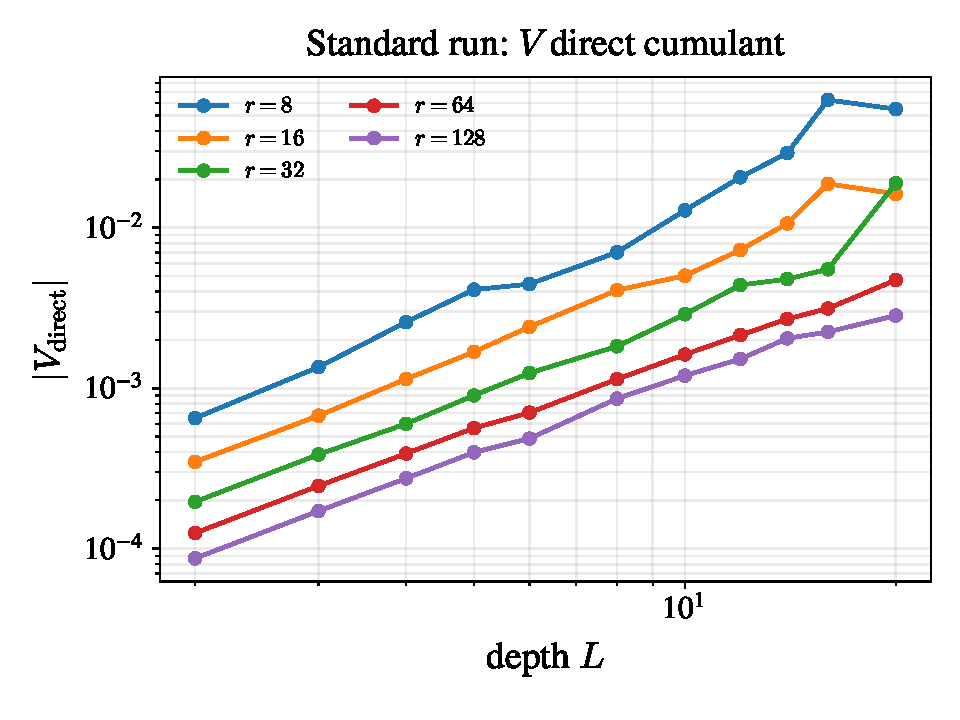
\includegraphics[width=\linewidth]{../../data/feynman/true_finite_ntk_cumulants_very_long/cumulant_loglog_V_same_off.pdf}
\end{minipage}
\hfill
\begin{minipage}{0.32\linewidth}
\centering
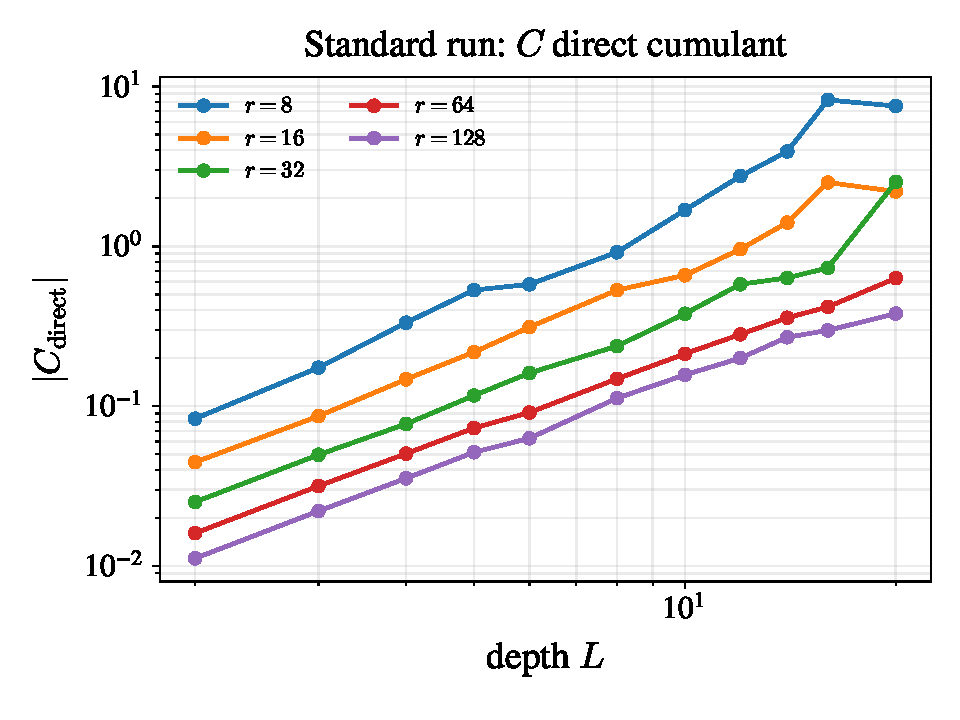
\includegraphics[width=\linewidth]{../../data/feynman/true_finite_ntk_cumulants_very_long/cumulant_loglog_C_same_off.pdf}
\end{minipage}
\hfill
\begin{minipage}{0.32\linewidth}
\centering
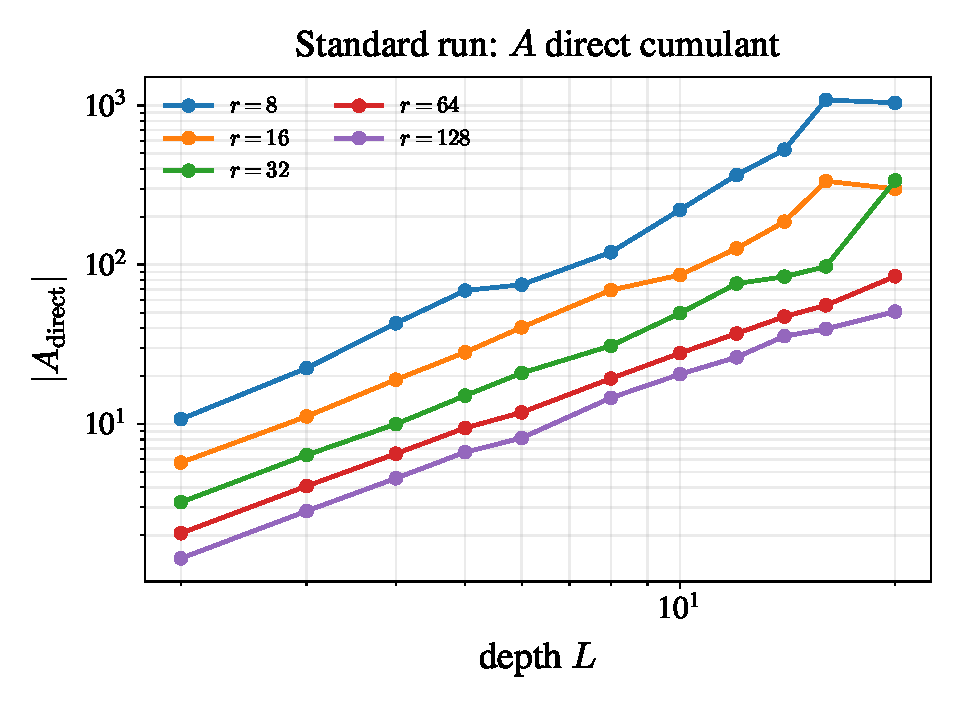
\includegraphics[width=\linewidth]{../../data/feynman/true_finite_ntk_cumulants_very_long/cumulant_loglog_A_same_off.pdf}
\end{minipage}
\caption{Log-log direct finite-network cumulant magnitudes. These plots complement the normalized-ratio plots in the main text.}
\label{fig:appendix-cumulant-loglog}
\end{figure}

\begin{figure}[h]
\centering
\begin{minipage}{0.32\linewidth}
\centering
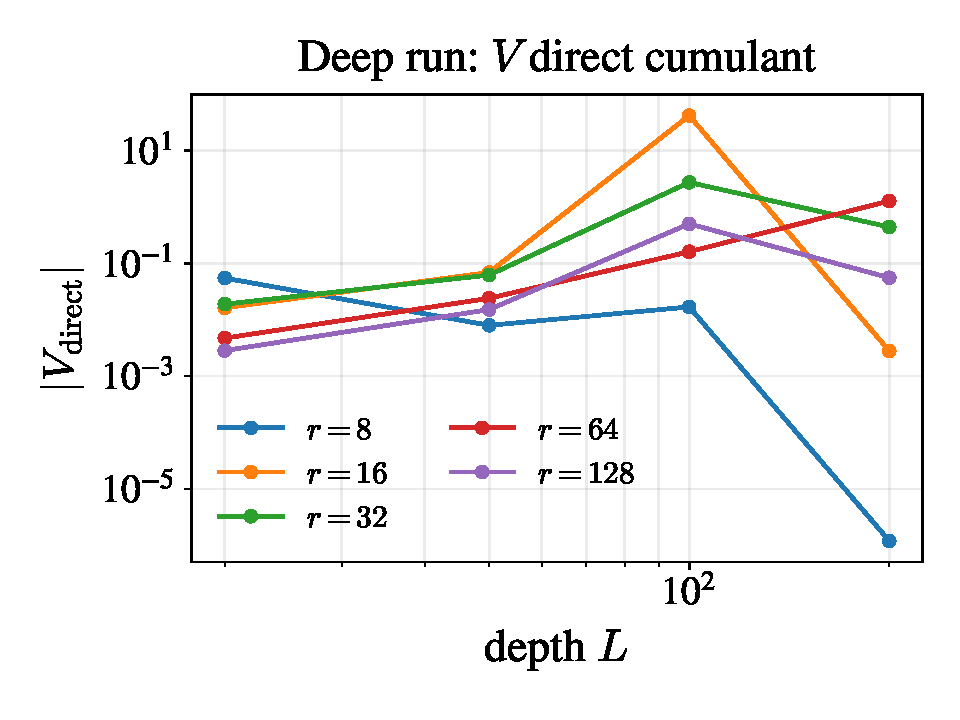
\includegraphics[width=\linewidth]{../../data/feynman/true_finite_ntk_cumulants_depth_20_50_100_200/cumulant_loglog_V_same_off.pdf}
\end{minipage}
\hfill
\begin{minipage}{0.32\linewidth}
\centering
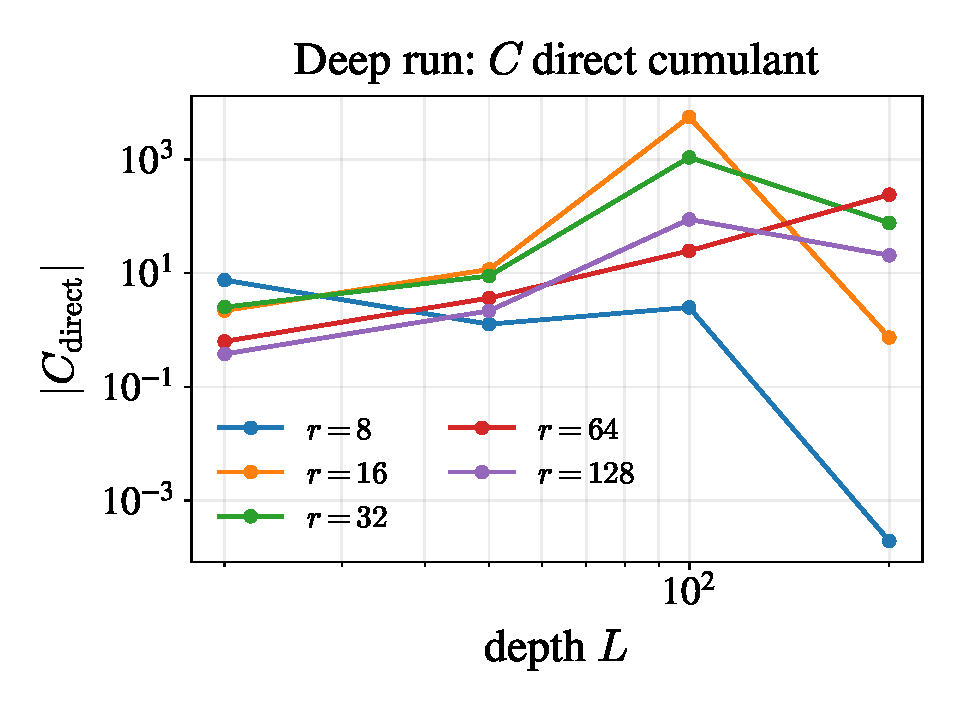
\includegraphics[width=\linewidth]{../../data/feynman/true_finite_ntk_cumulants_depth_20_50_100_200/cumulant_loglog_C_same_off.pdf}
\end{minipage}
\hfill
\begin{minipage}{0.32\linewidth}
\centering
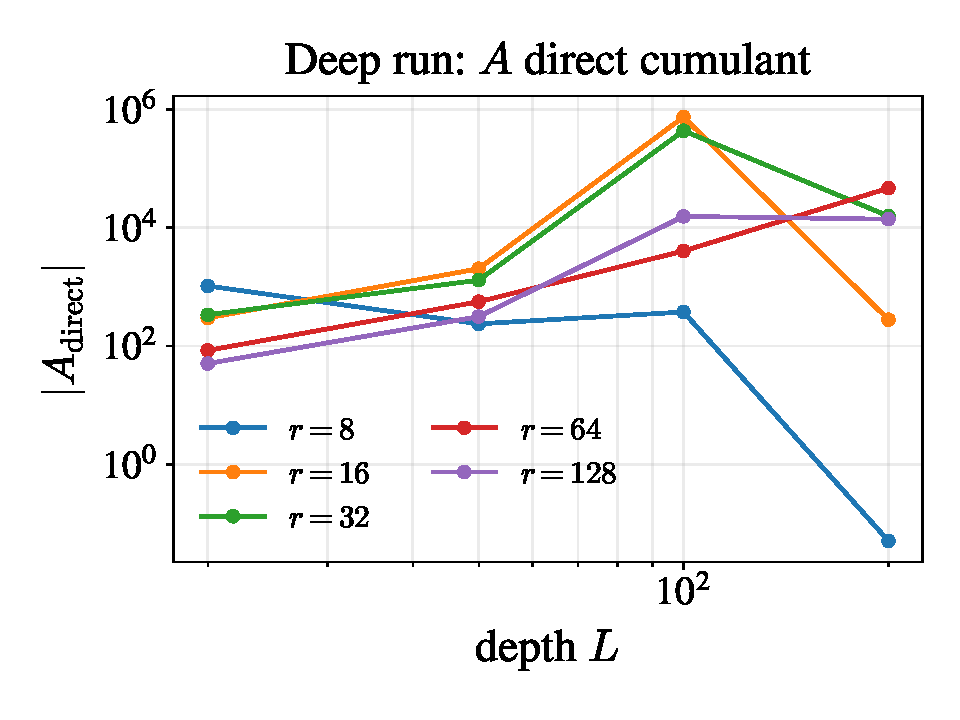
\includegraphics[width=\linewidth]{../../data/feynman/true_finite_ntk_cumulants_depth_20_50_100_200/cumulant_loglog_A_same_off.pdf}
\end{minipage}
\caption{Deep-run log-log cumulant magnitudes for \(L\in\{20,50,100,200\}\). These plots are a stress test rather than a clean asymptotic fit: they reveal where finite-network cumulants become dominated by finite-depth and sampling effects.}
\label{fig:appendix-deep-cumulant-loglog}
\end{figure}

\end{document}
